\documentclass[12px]{article}
\usepackage[utf8x]{inputenc}
\usepackage[portuges]{babel}
\usepackage[svgnames]{xcolor}
\usepackage{graphicx}
\usepackage{a4wide}
\usepackage{float}
\usepackage[export]{adjustbox}
\usepackage{spverbatim}
\usepackage{hyperref}
\usepackage{enumitem}

\setdescription{leftmargin=\parindent,labelindent=\parindent}

\newcommand*{\plogo}{\fbox{$\mathcal{PL}$}}
\newcommand*{\titleTH}{\begingroup
\raggedleft
\vspace*{\baselineskip}

{\Large Universidade do Minho}\\[0.167\textheight]
{\LARGE\bfseries Projeto Integrado}\\[\baselineskip]
{\Huge Gestão de Trabalhos Práticos}\\[\baselineskip]
{\Large \textit{Engenharia de Linguagens 13/14}}\par

\vfill

\Large{André Santos pg25329\\Daniel Carvalho a61008\\Ricardo Branco pg25339}\par

\vspace*{3\baselineskip}
\endgroup}

\begin{document}
\thispagestyle{empty}
\titleTH
\newpage

\section{Resumo}
  Este relatório cobre todo o processo de planeamento, desenvolvimento e
  documentação de um sistema que resolva um problema abordado na UCE de
  Engenharia de Linguagens na forma de Projecto Integrado, nomeadamente
  a gestão de trabalhos práticos académicos desde a sua criação pelos docentes, à resolução pelos alunos
  e à publicação dos mesmos ao resto da comunidade \textit{online}.

  A abordagem na resolução deste projecto passa por aliar todos os conhecimentos
  adquiridos nos módulos integrantes de Engenharia de Linguagens, passando por
 Engenharia Gramatical, Scripting no Processamento de Linguagem Natural, Processamento
 Estruturado de Documentos e Análise e Transformação de Software.

 Neste sentido pretende-se aliar ao desenvolvimento deste sistema conhecimentos
 como gramáticas de atributos, ambientes de desenvolvimento estruturais e
 orientados à semântica, representação de manipulação de conhecimento com
 eficiência, automatização de tarefas e transformações, utilização de expressões
 regulares, linguagens DSL, corpora, automatização de testes para diferentes
 linguagens de programação, manipulação de documentos estruturados, utilização
 de XML, XSL e XSLFO, documentos anotados, publicação de conhecimento na web,
 entre outros.

\newpage

\tableofcontents
\newpage

\section{Introdução}

\section{Plano de trabalho}
Tendo em conta a dimensão da aplicaçãoewf,,,,,,,,,,,,,,,,,,, foi criado um plano de trabalho onde mapeámos as tarefas
de desenvolvimento no tempo de forma contínua tornado assim possível adaptar um ritmo de trabalho
consistente com os prazos de entrega de cada fase e então cumprir as metas do projecto.
Nesse sentido dividimos o projecto em três fases, sendo elas o planeamento e análise de requisitos, o
desenvolvimento e a documentação.
No que diz respeito à fase de planeamento e análise de requisitos, esta fase engloba todo o levantamento 
de funcionalidades assim como todo o planeamento e estruturação do projecto como
criação do modelo de domínio, diagrama de classes, modelação do repositório de dados,
análise da concorrência, plano tecnológico, etc.
Para esta fase de planeamento, análise e modelação foi criado um plano de um mês onde todas as tarefas 
teriam de estar concluídas. Na imagem seguinte é possível ver um diagrama de Gannt com
o planeamento inicial.



\begin{figure}[htbp] 
	\centering
	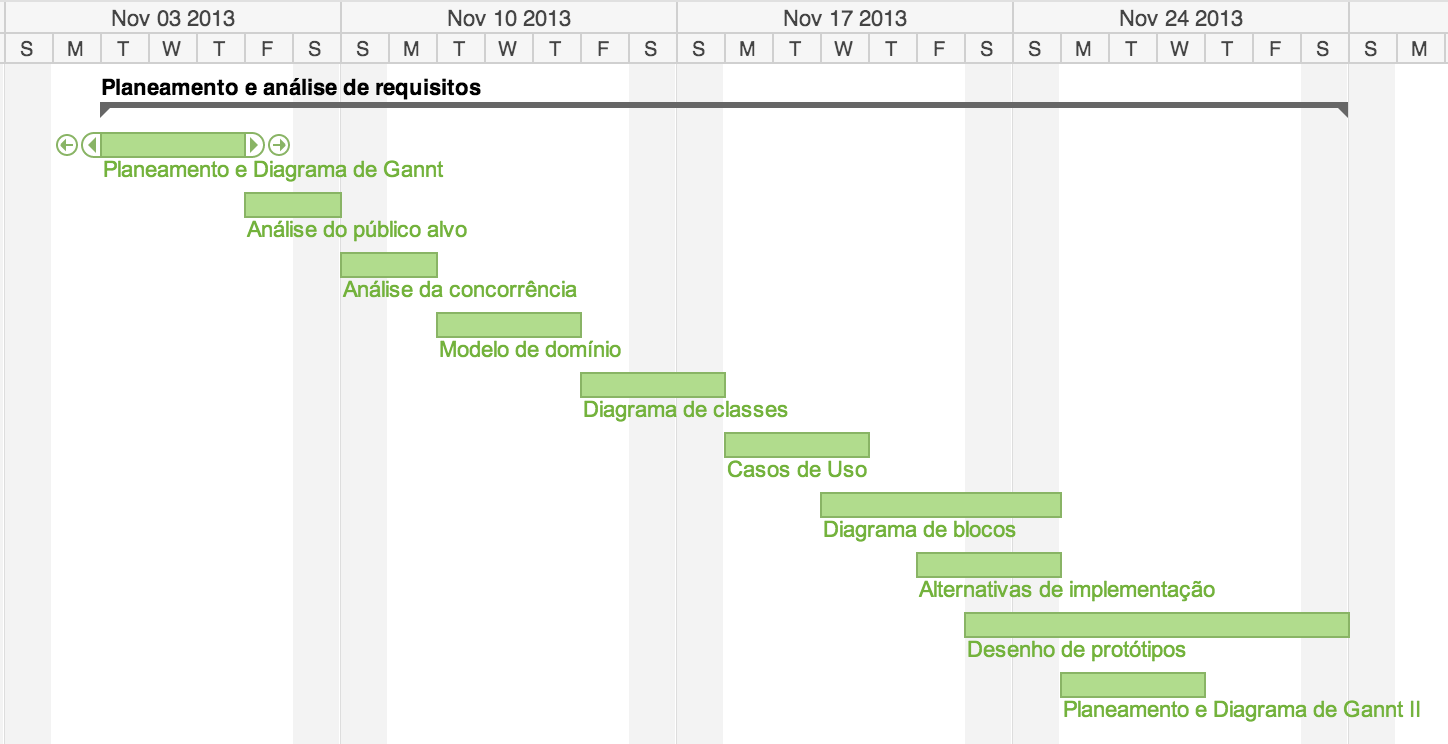
\includegraphics[width=1\textwidth]{images/plano_trabalho_1.png}
 	\caption{Diagrama de Gannt para o planeamento e análise de requisitos}
 	\label{fig: workplan1}
\end{figure}


De seguida, prosseguindo para o planeamento da fase de desenvolvimento após 
analisar as funcionalidades e modelar o sistema  é altura de começar a 
prototipar a aplicação e começar a iterar sobre as funcionalidades a 
implementar. Neste sentido englobámos aqui tarefas como prototipagem em HTML, 
criação de migrações na modelação da base dados, modelação das entidades a 
representar (modelos) na forma da arquitectura MVC seguindo-se a implementação dos 
controladores e visões tendo como base as funcionalidades a desenvolver para o 
sistema.  Nesta fase pretende-se tornar a aplicação capaz de suportar os seus 
utilizadores (não registados, docentes e alunos) das tarefas de gestão de UCs, 
projectos, grupos, submissões, assim como consulta e disponibilização de 
projectos. De forma a tornar a aplicação o mais robusta possível planeamos um 
espaço temporal dedicado a testes de usabilidade e funcionalidade de forma a 
corrigir todos os pormenores que possam ter um impacto negativo.


\begin{figure}[htbp] 
	\centering
	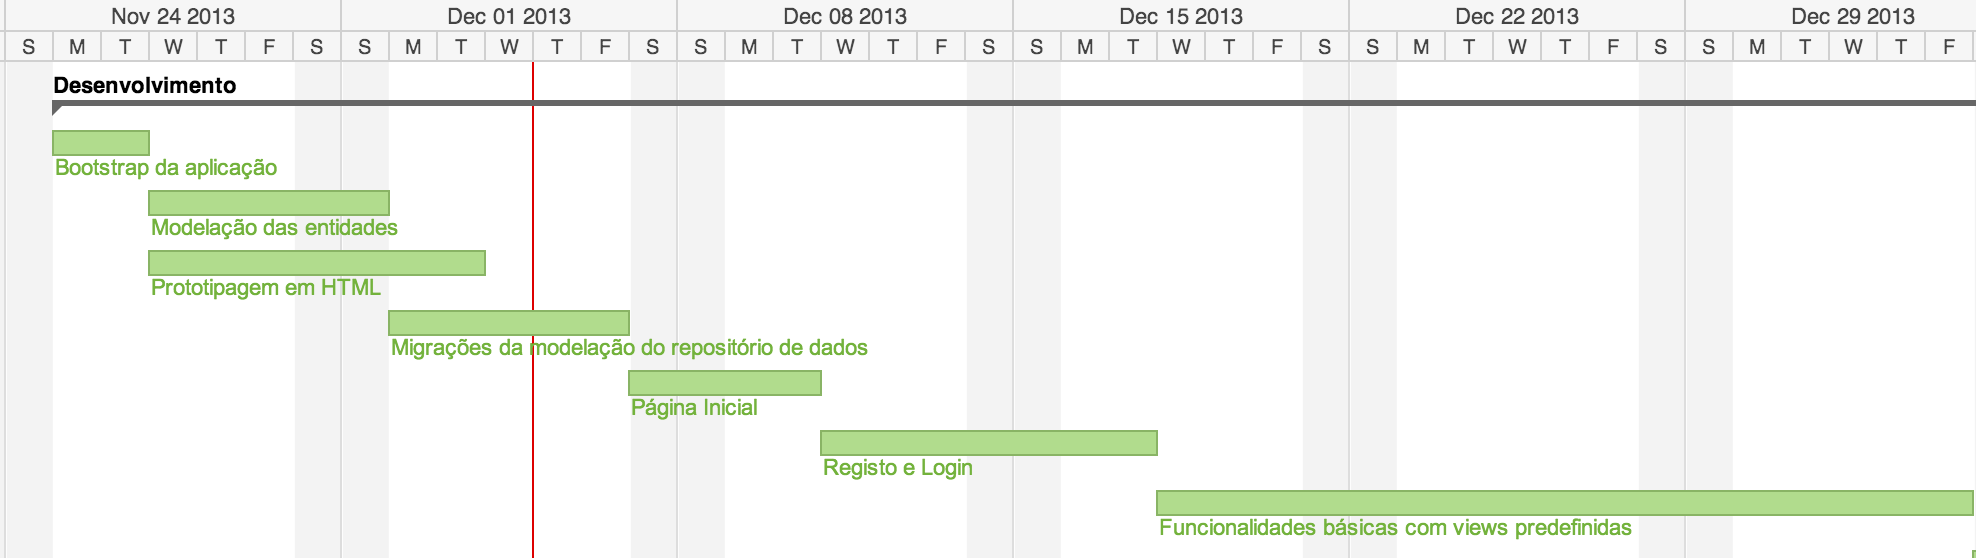
\includegraphics[width=1\textwidth]{images/plano_trabalho_2.png}
 	\caption{Diagrama de Gannt para o desenvolvimento I}
 	\label{fig: workplan2}
\end{figure}

\begin{figure}[htbp] 
	\centering
	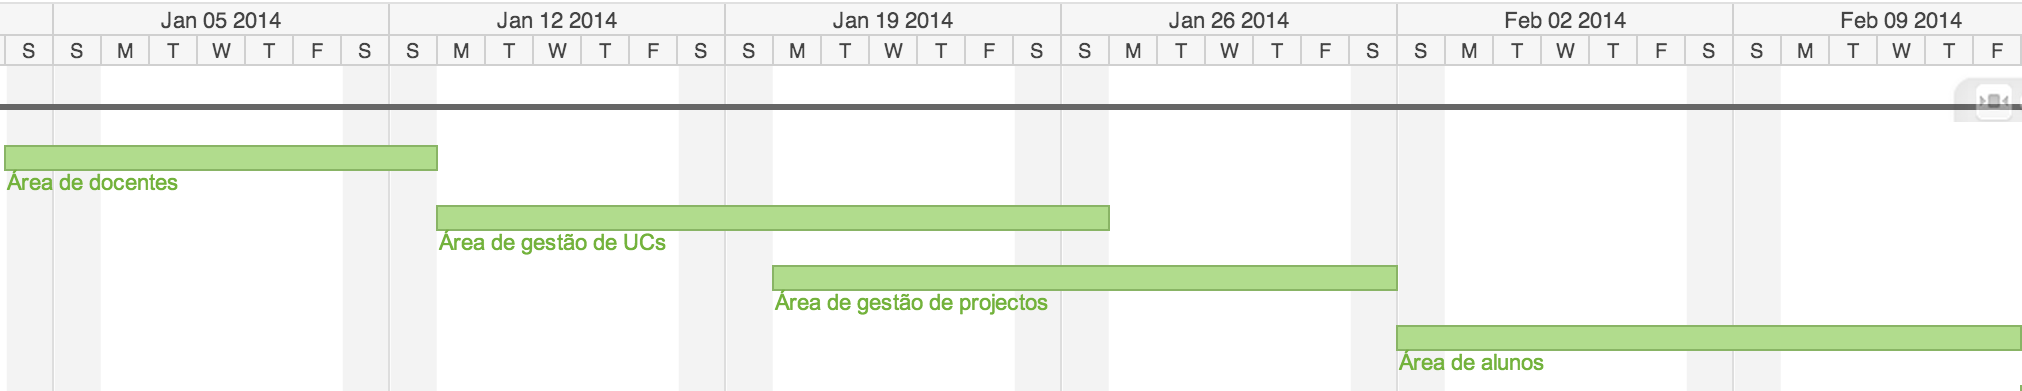
\includegraphics[width=1\textwidth]{images/plano_trabalho_3.png}
 	\caption{Diagrama de Gannt para o desenvolvimento II}
 	\label{fig: workplan3}
\end{figure}

\begin{figure}[htbp] 
	\centering
	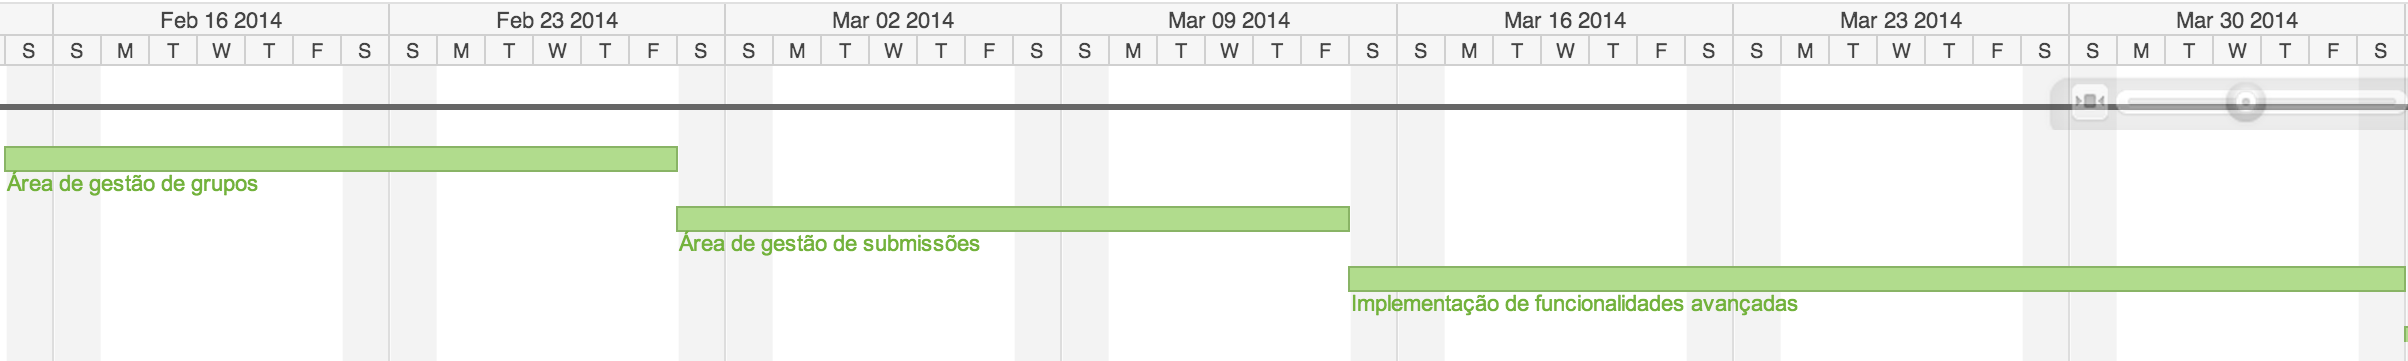
\includegraphics[width=1\textwidth]{images/plano_trabalho_4.png}
 	\caption{Diagrama de Gannt para o desenvolvimento III}
 	\label{fig: workplan4}
\end{figure}

\begin{figure}[htbp!] 
	\centering
	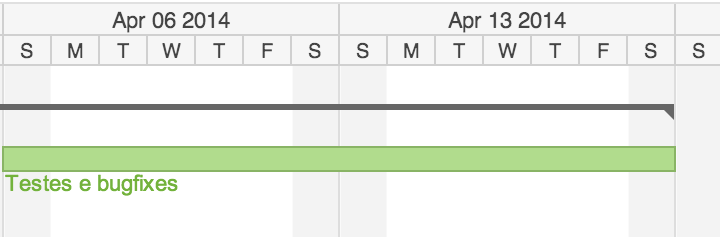
\includegraphics[width=1\textwidth]{images/plano_trabalho_5.png}
 	\caption{Diagrama de Gannt para o desenvolvimento IV}
 	\label{fig: workplan5}
\end{figure}


Por fim, terminámos com a fase de documentação onde será feita toda a descrição 
do sistema desenvolvido em termos de funcionalidades e implementação de forma a 
possibilitar a consulta tanto aos interessados em utilizar a aplicação bem como 
de forma a suportar a possível necessidade de manutenção da aplicação. Desta 
forma qualquer um pode entender todo o sistema na sua plenitude através da 
documentação criada. Para esta fase reservou-se o restante tempo disponível até 
à entrega final do projecto.


\section{Análise do problema}

No meio académico, principalmente em áreas mais focadas numa vertente prática, muitas vezes
os alunos são postos à prova através de trabalhos práticos. Neste caso, após a avaliação, os trabalhos
práticos são arquivados pelos docentes e esquecidos permanentemente numa prateleira, até um dia
serem deitados fora.

No sentido de promover a investigação e a partilha de conhecimento, torna-se não só necessário
criar uma plataforma de gestão de disciplinas universitárias e os seus trabalhos práticos, como também
tornar possível a partilha de todo o conhecimento que é inevitavelmente inerente aos resultados
do desenvolvimento destes.

No momento as ferramentas que existem no mercado, se por um lado permitem toda a gestão de
unidades curriculares de uma universidade, pecam por se focarem por um funcionamento fechado
para dentro da instituição e consequentemente fechado para dentro dos cursos e das unidades curriculares.
Nesse sentido o sistema retratado neste relatório, preenche a lacuna existente entre o que é desenvolvido
num âmbito académico e o resto da população.

Como resultado deste tipo de ponte entre os dois mundos, espera-se conseguir manter uma plataforma
que não só incentive a investigação tanto dentro do mundo académico, como profissional e individual,
como também incentive a partilha de conhecimento e fomente o desenvolvimento das
áreas de atuação condizentes com cada trabalho prático disponível na
plataforma.

Para além disso, torna-se imperativo criar um modelo genérico de publicação de
trabalhos práticos para dessa forma se tornar muito mais acessível o consumo de
informação para os utilizadores da plataforma.

No entanto também se torna necessário o foco no lado mais académico e das
necessidades dos docentes e alunos. Neste sistema todo o processo de
interatividade entre os utilizadores e a aplicação, permite tanto aos docentes
como aos alunos realizarem a gestão das suas unidades curriculares e trabalhos
práticos criando assim um sistema que cumpre as necessidades académicas internas dos docentes
e alunos bem como estabelece um ponto de ligação entre a comunidade académica e
o trabalho desenvolvido nesse meio, e o resto das pessoas com interesse nas
áreas abrangidas pelos projetos disponíveis.

\newpage

\section{Análise de requisitos}

Identificado o problema, pretende-se assim desenvolver um sistema de informação para gestão de trabalhos práticos. O sistema oferecerá um conjunto de funcionalidades e facilidades aos docentes e alunos em todo o processo de entrega de um trabalho prático, desde a gestão da unidade curricular até à publicação das avaliações.\\

Identifica-se à partida 3 grupos de utilizadores com funcionalidades e objetivos diferentes em todo o processo.\\

O primeiro grupo de utilizadores são os \textbf{alunos}, para estes pretende-se oferecer a possibilidade de submeterem projetos práticos de uma forma simples e facilitada. As submissões poderão ser efetuadas individualmente ou em grupos conforme o especificado pelo docente. O aluno terá acesso a um painel de gestão das suas unidades curriculares e projetos, poderá consultar todas as informações de um projeto e respetivas fases, gerir facilmente os seus grupos de trabalho, consultar o seu histórico de entregas e consultar em diferentes formatos as suas avaliações dos projetos e/ou fases. Pretende-se ainda que o aluno tenha a possibilidade de ser notificado de todas as alterações nos projetos que faz parte, através de avisos do sistema ou emails. Estas notificações serão também importantes para informar o aluno da aproximação dos prazos de entrega dos projetos das suas unidades curriculares.\\
No processo de submissão de um projeto, o sistema, deverá ser capaz de facilitar a criação do \textit{Project Record} do pacote enviado, assim como identificar e notificar falhas na submissão, tais como não conter todos os ficheiros obrigatórios ou não gerar o executável pretendido. Neste caso os alunos poderão receber no email essa informação para assim submeterem uma versão corrigida.
Um aluno terá também a possibilidade de tornar o projeto desenvolvido público.\\

O segundo grupo de utilizadores são os \textbf{docentes}, numa primeira componente estes utilizadores poderão criar e gerir unidades curriculares e todas as informações adjacentes a estas, um docente de uma unidade curricular pode adicionar docentes responsáveis, adicionar alunos e associá­-los a diferentes turnos. Dentro da gestão de uma unidade curricular um docente será capaz de criar projetos devidamente documentados (organizados ou não em diferentes fases), podendo ainda especificar ficheiros obrigatórios, executável obrigatório e ficheiros de teste para facilitar a correção dos mesmos. Estes testes serão executados no programa enviado e serão guardadas as diferenças do output obtido para o output esperado. Dentro do painel de gestão de um projeto o docente poderá consultar as entregas dos diferentes grupos e avaliar as entregas por grupo ou individualmente. Depois de avaliadas as entregas, o docente, poderá gerar automaticamente as pautas do projeto e/ou fase e publicar para os alunos da unidade curricular.
Numa fase final, o docente poderá tornar o projeto (enunciado e especificações do problema) público.\\

Para além dos docentes e dos alunos, o nosso sistema permitirá uma procura e consulta de projetos públicos desenvolvidos a \textbf{utilizadores não registados}.\\

Pretende-se no desenvolvimento do sistema simplificar todas as tarefas dos utilizadores alvo do sistema, e proporcionar um sistema flexível que possa ser utilizado por um abrangente número de utilizadores.\\

Nesse seguimento o sistema procurará ser flexível, não se restringindo a apenas uma abordagem nem sendo demasiado genérico, procurar-se-á definir abordagens mais específicas, mas sempre com opções mais genéricas para englobar casos menos comuns. É exemplo disso a geração automática do \textit{Project Record} do pacote enviado, em casos mais específicos o ficheiro poderá ser entregue pelo utilizador, no entanto em outros casos torna-se necessário auxiliar na geração desse mesmo ficheiro para assegurar que todos os pacotes enviados estão em conformidade com a estrutura esperada de um pacote. O sistema também procurará simplificar processos organizacionais, como facilitar a criação de uma unidade curricular identificando apenas nome, instituição, curso e ano letivo. O facto de uma unidade curricular estar associada a um ano letivo ajuda a nível organizacional e permite que não seja necessária a transferência de alunos e docentes entre anos letivos. Procurará também simplificar processos de validação das entregas através das restrições de ficheiros obrigatórios e nome do executável. Ser capaz de automatizar a avaliação através dos testes no sistema e geração de pautas automáticas e de gerir mais facilmente grupos de trabalho e respetivas entregas.\\

O objetivo final é lançar um sistema bem focado onde cada grupo de utilizadores execute com facilidade as suas tarefas principais, perdendo o menor tempo possível em problemas secundários. 

\section{Concorrência e alternativas}

Uma das medidas efetuadas durante o planeamento da aplicação foi a análise de concorrência e o estudo das alternativas existentes. Desta forma foi possível adicionar mais funcionalidades à aplicação de forma a que esta fosse o mais completa possível.

\subsection{Concorrência}
\label{sub:concorrencia}

De todas as aplicações concorrentes, as que mais se destacam são os Sistemas de Gestão de Aprendizagem (\emph{SGA}),também conhecidas por \emph{Learning Management Systems} - \emph{LMS}. Dentro dos \emph{SGA} imperam as seguintes aplicações:
\begin{itemize}
	\item \emph{Blackboard}
	\item \emph{Moodle}
	\item \emph{Studifi}
	\item \emph{Haiku LMS}
\end{itemize}

\subsubsection{Blackboard}
\label{ssub:blackboard}

\begin{figure}[H]
        \centering
        
\includegraphics[width=0.5\textwidth]{images/concorrencia/blackboard.jpg}
         \caption{\emph{Blackboard}}
         \label{fig: blackboard}
\end{figure}

A aplicação \href{http://www.blackboard.com}{\emph{Blackboard}} é composta por quatro tipos de utilizadores:
\begin{description}
	\item[Aluno] Um aluno pode submeter projetos, inscrever-se em grupos e consultar a informação disponibilizada pelos professores.
	\item[Professores] Um professor pode criar projetos e fazer avaliações qualitativas e quantitativas dos trabalhos enviados. Os projetos criados podem ter correção automática.
	\item[Técnicos] Os técnicos são responsáveis pela manutenção da aplicação.
	\item[Supervisores] Os supervisores fazem a gestão de cursos, disciplinas, docentes e alunos. Estes também podem gerar estatísticas do sistema.
\end{description}

Os projetos criados na \emph{Blackboard} não estão disponíveis para o público. Também não existe a noção de turnos, sendo estes substituídos pelos grupos. Os grupos são criados dentro da disciplina e um aluno pode estar inscrito em múltiplos grupos.

\subsubsection{Moodle}
\label{ssub:moodle}
\begin{figure}[H]
        \centering
        
\includegraphics[width=0.5\textwidth]{images/concorrencia/moodle.jpg}
         \caption{\emph{Moodle}}
         \label{fig: moodle}
\end{figure}
A aplicação \href{http://www.moodle.org}{\emph{Moodle}} é composta por três tipos de utilizadores:

\begin{description}
	\item[Alunos] Os alunos podem submeter projetos e consultar a informação disponibilizada pelos professores.
	\item[Professores] Os professores podem criar projetos e fazer uma avaliação quantitativa dos projetos enviados. Os projetos criados podem ter correção automática.
	\item[Administradors] Os Administradores são responsáveis pela manutenção da aplicação. Também são responsáveis por fazer a gestão dos utilizadores existentes.
\end{description}


Um dos problemas do \emph{Moodle} é a inexistência de grupos e de turnos. Quanto a projetos públicos apenas se estes forem inseridos manualmente pelos alunos nos seus portefólios.

\subsubsection{Studifi}
\label{ssub:studifi}

\begin{figure}[H]
        \centering
        
\includegraphics[width=0.5\textwidth]{images/concorrencia/studifi.png}
         \caption{\emph{Studifi}}
         \label{fig: studifi}
\end{figure}

A aplicação \href{https://studifi.com/}{\emph{Studifi}} é composta por três tipos de utilizadores:

\begin{description}
	\item[Alunos] Os alunos podem submeter projetos e consultar a informação disponibilizada pelos professores.
	\item[Professores] Os professores podem criar exercícios que são avaliados automaticamente e podem criar projetos.
	\item[Administradors] Os Administradores são responsáveis pela manutenção da aplicação. Também são responsáveis por fazer a gestão dos utilizadores existentes.
\end{description}

No \emph{Studifi} os exercícios não estão disponíveis para o público. Uma das características que se destaca nesta aplicação é a existência de controlo de versões nos ficheiros submetidos.

\subsubsection{Haiku LMS}
\label{ssub:haiku_lms}

\begin{figure}[H]
        \centering
        
\includegraphics[width=0.5\textwidth]{images/concorrencia/haiku.png}
         \caption{\emph{Haiku LMS}}
         \label{fig: studifi}
\end{figure}

A aplicação \href{http://www.haikulearning.com/}{\emph{Haiku LMS}} é composta por três tipos de utilizadores:

\begin{description}
	\item[Alunos] Os alunos podem submeter projetos e consultar a informação disponibilizada pelos professores.
	\item[Professores] Os professores podem criar projetos e exercícios e gerir pautas de avaliação.
	\item[Instituições de ensino] Responsáveis pela gestão de cursos e disciplinas da instituição.
\end{description}

\subsection{Alternativas}
\label{sub:alternativas}

No que diz ao respeito às alternativas, estas são divididas em cinco situações:
\begin{itemize}
	\item Submissão de trabalhos

	\begin{description}
		\item[Submissão via \emph{mail}] O aluno envia um \emph{mail} com o trabalho para o \emph{mail} de um docente. Muitas vezes com um assunto especifico para que o docente possa filtrar o \emph{mail} e obter os vários trabalhos enviados.
		\item[Partilha de \emph{links}] O aluno faz \emph{upload} do seu trabalho para um servidor externo(\emph{github,dropbox,etc}) e partilha o \emph{link} com o docente.
		\item[Entrega de unidades de armazenamento] O aluno grava o seu trabalho numa unidade de armazenamento(\emph{Usb flash drive, cd/dvd, etc}) e entrega a respetiva unidade ao docente.
	\end{description}

	\item Gestão de pautas

	\begin{description}
		\item[Folhas de cálculo ou \emph{PDF}] É entre aos alunos um ficheiro com as notas do projeto. Muitas vezes a pauta entregue não refere a qualidade do trabalho.
		\item[Vitrinas] O docente imprime as notas finais e afixa-as numa vitrina do estabelecimento de ensino.
	\end{description}

	\item Correção automática

		\begin{description}
			\item[Script] Fica ao critério do docente, as funcionalidades desse emph{script}, isto é se o emph{script} criado verifica por exemplo extensões de ficheiros ou até mesmo se os ficheiros enviados correspondem a um determinado emph{output} para um certo \emph{input}.
		\end{description}
	\item Inscrições de grupos

	\begin{description}
		\item[\emph{Mail}] Um responsável do grupo envia um \emph{mail} ao docente com a constituição do grupo. Este \emph{mail} pode ficar sujeito as mesma regras que a submissão de trabalhos via \emph{mail}.
		\item[Entrega do trabalho] O grupo só fica registado e o docente só tem conhecimento desta após a entrega do trabalho.
		\item[Aviso com presença] Um elemento do grupo ou então todos os elementos notificam o docente em frente deste.
	\end{description}

	\item Gestão de grupos

	\begin{description}
		\item[Documento] O docente possui um documento com a constituição dos grupos e de outras informações relativas a esse grupo como por exemplo as notas dos trabalhos
	\end{description}

\end{itemize}

\newpage

\section{Casos de estudo}
De forma a verificar a viabilidade da aplicação decidiu-se usar três casos reais.

\subsection{Engenharia de Linguagens} % (fold)
\label{sub:engenharia_de_linguagens}

% subsection engenharia_de_linguagens (end)

No primeiro caso pretende-se que haja uma plataforma para a submissão do Projeto Integrado de Engenharia de Linguagens do Mestrado em Engenharia Informática da Universidade do Minho.
Engenharia de Linguagens tem um turno e quatro docentes.
Quanto ao Projeto Integrado, este tem que ser feito por grupos com o máximo de três elementos, existem quatro fases de entrega(as 3 primeiras tem uma nota qualitativa e a última fase vale 20 valores). Relativamente à entrega, em cada fase é obrigatório entregar um relatório e um conjunto de slides usados na apresentação, na última fase além do relatório, é para enviar o código desenvolvido assim como outros ficheiros que o grupo ache relevante.
O processo começa com o registo do docente responsável, caso este já possuia uma conta tem efetuar login na aplicação. Após o login é necessário criar a cadeira de Engenharia de Linguagens, durante este processo será necessário preencher campos relativos ao nóme da instituição e do curso, caso um destes já exista a disciplina será associada aos campos existentes. No fim de criar a disciplina, o docente será encaminhado para o painel da disciplina criada. Dentro do painel da disciplina, o docente responsável pode adicionar docentes à disciplina.
Procede-se para a criação do projeto. Ao criar um novo projeto o docente adiciona o enunciado, adiciona as várias fases do projeto, indica que os grupos só podem ter três elementos. Em cada fase indica que tem que ser enviado um relatório e os slides da apresentação em formato \emph{PDF}. Por fim tem a opção de lançar o projeto ou se apenas o quer deixar visivel para o resto da equipa docente, para o caso de haverem alterações.Após o projeto estar criado o docente é encaminhado para o painel do projeto.
Um aluno uma vez registado e autenticado inscreve-se na cadeira e acede ao painel do projeto. No painel do projeto cria o seu grupo e faz uma submissão. É então reencaminhado para um formulario onde escreve um resumo do trabalho feito e envia os ficheiros necessários, concluindo assim a submissão.
Voltando ao docente, este acede novamente ao painel do projeto e abre a página de entrega de um projeto submetido. Após analizar o relatório ou qualquer outro ficheiro enviado, carrega em avaliar e atribui a nota ao grupo ou a cada elemento individualmente, podendo também adicionar comentários sobre a nota atribuida.


\subsection{Estatística} % (fold)
\label{sub:estat_stica}

% subsection estat_stica (end)

No segundo caso tem-se como exemplo um projeto da cadeira de Estatística do curso de Economia. Esta cadeira tem quatro turnos e dois docentes. Quanto ao projeto tem que ser feito em grupos de dois ou três elementos, restringido a alunos do mesmo turno, tem apenas uma fase, existe um ficheiro com dados para auxilio da realização do projeto e no momento da entrega além do relatório tem-se que enviar os resultados obtidos no \emph{SPSS} que estão no formato \emph{SAV}.
O processo começa pelo registo da cadeira no sistema após o registo e identificação do docente. Assumindo que todos os alunos já se inscreveram na disciplina é feito a inscrição dos alunos em cada turno por parte do docente. De seguida cria-se o projeto no qual se indica o enunciado do projeto, o ficheiro de dados, restringe-se os grupos de forma a que estes sejam constituidos por elementos do mesmo turno e que a dimensão deste seja de dois a três elementos e indica-se quais os ficheiros obrigatórios no momento da entrega. Por último os alunos submetem o projeto feito e o docente indica a nota do mesmo tal como acontece no primeiro caso.

\subsection{Desafios de Proramação da Universidade do Minho} % (fold)
\label{sub:desafios_de_prorama_o_da_universidade_do_minho}

% subsection desafios_de_prorama_o_da_universidade_do_minho (end)

No terceiro e último caso pretende-se submeter os desafios algorítmicos dos Desafios de Programação da Universidade do Minho (DPUM). Estes desafios são feitos individualente e são corregidos automáticamente pela aplicação. Não é necessário entregar relatório e não existe data limite de submissão.
Quanto aos Desafios de Programação da Universidade é dirigido por um único docente e não existem turnos. Na submissão de um desafio é obrigatório que haja uma \emph{Makefile} e que o nome do executável tem que ser igual o ao nome indicado pelo docente.
Assumindo que já existe o registo e autenticação do docente no sistema, procede-se para o registo do DPUM no sistema, o campo referente ao curso é deixado em branco.
Na criação de um desafio indica-se que se pretende que haja correção automática, faz-se upload dos ficheiros de \emph{input} e \emph{output} e que os grupos sejam de um único elemento. Para o aluno no momento da submissão não é necessário criar grupo. Após a submissão de um desafio é enviado um \emph{mail} para o aluno com os resultados da correção automática.





\section{Arquitetura do sistema}
\subsection{Modelo OAIS}
O nosso sistema será construido seguindo as orientações do modelo OAIS \textit{(Open Archival Information System)} da Figura ~\ref{fig:oais}

\begin{figure}[H] 
  \centering
  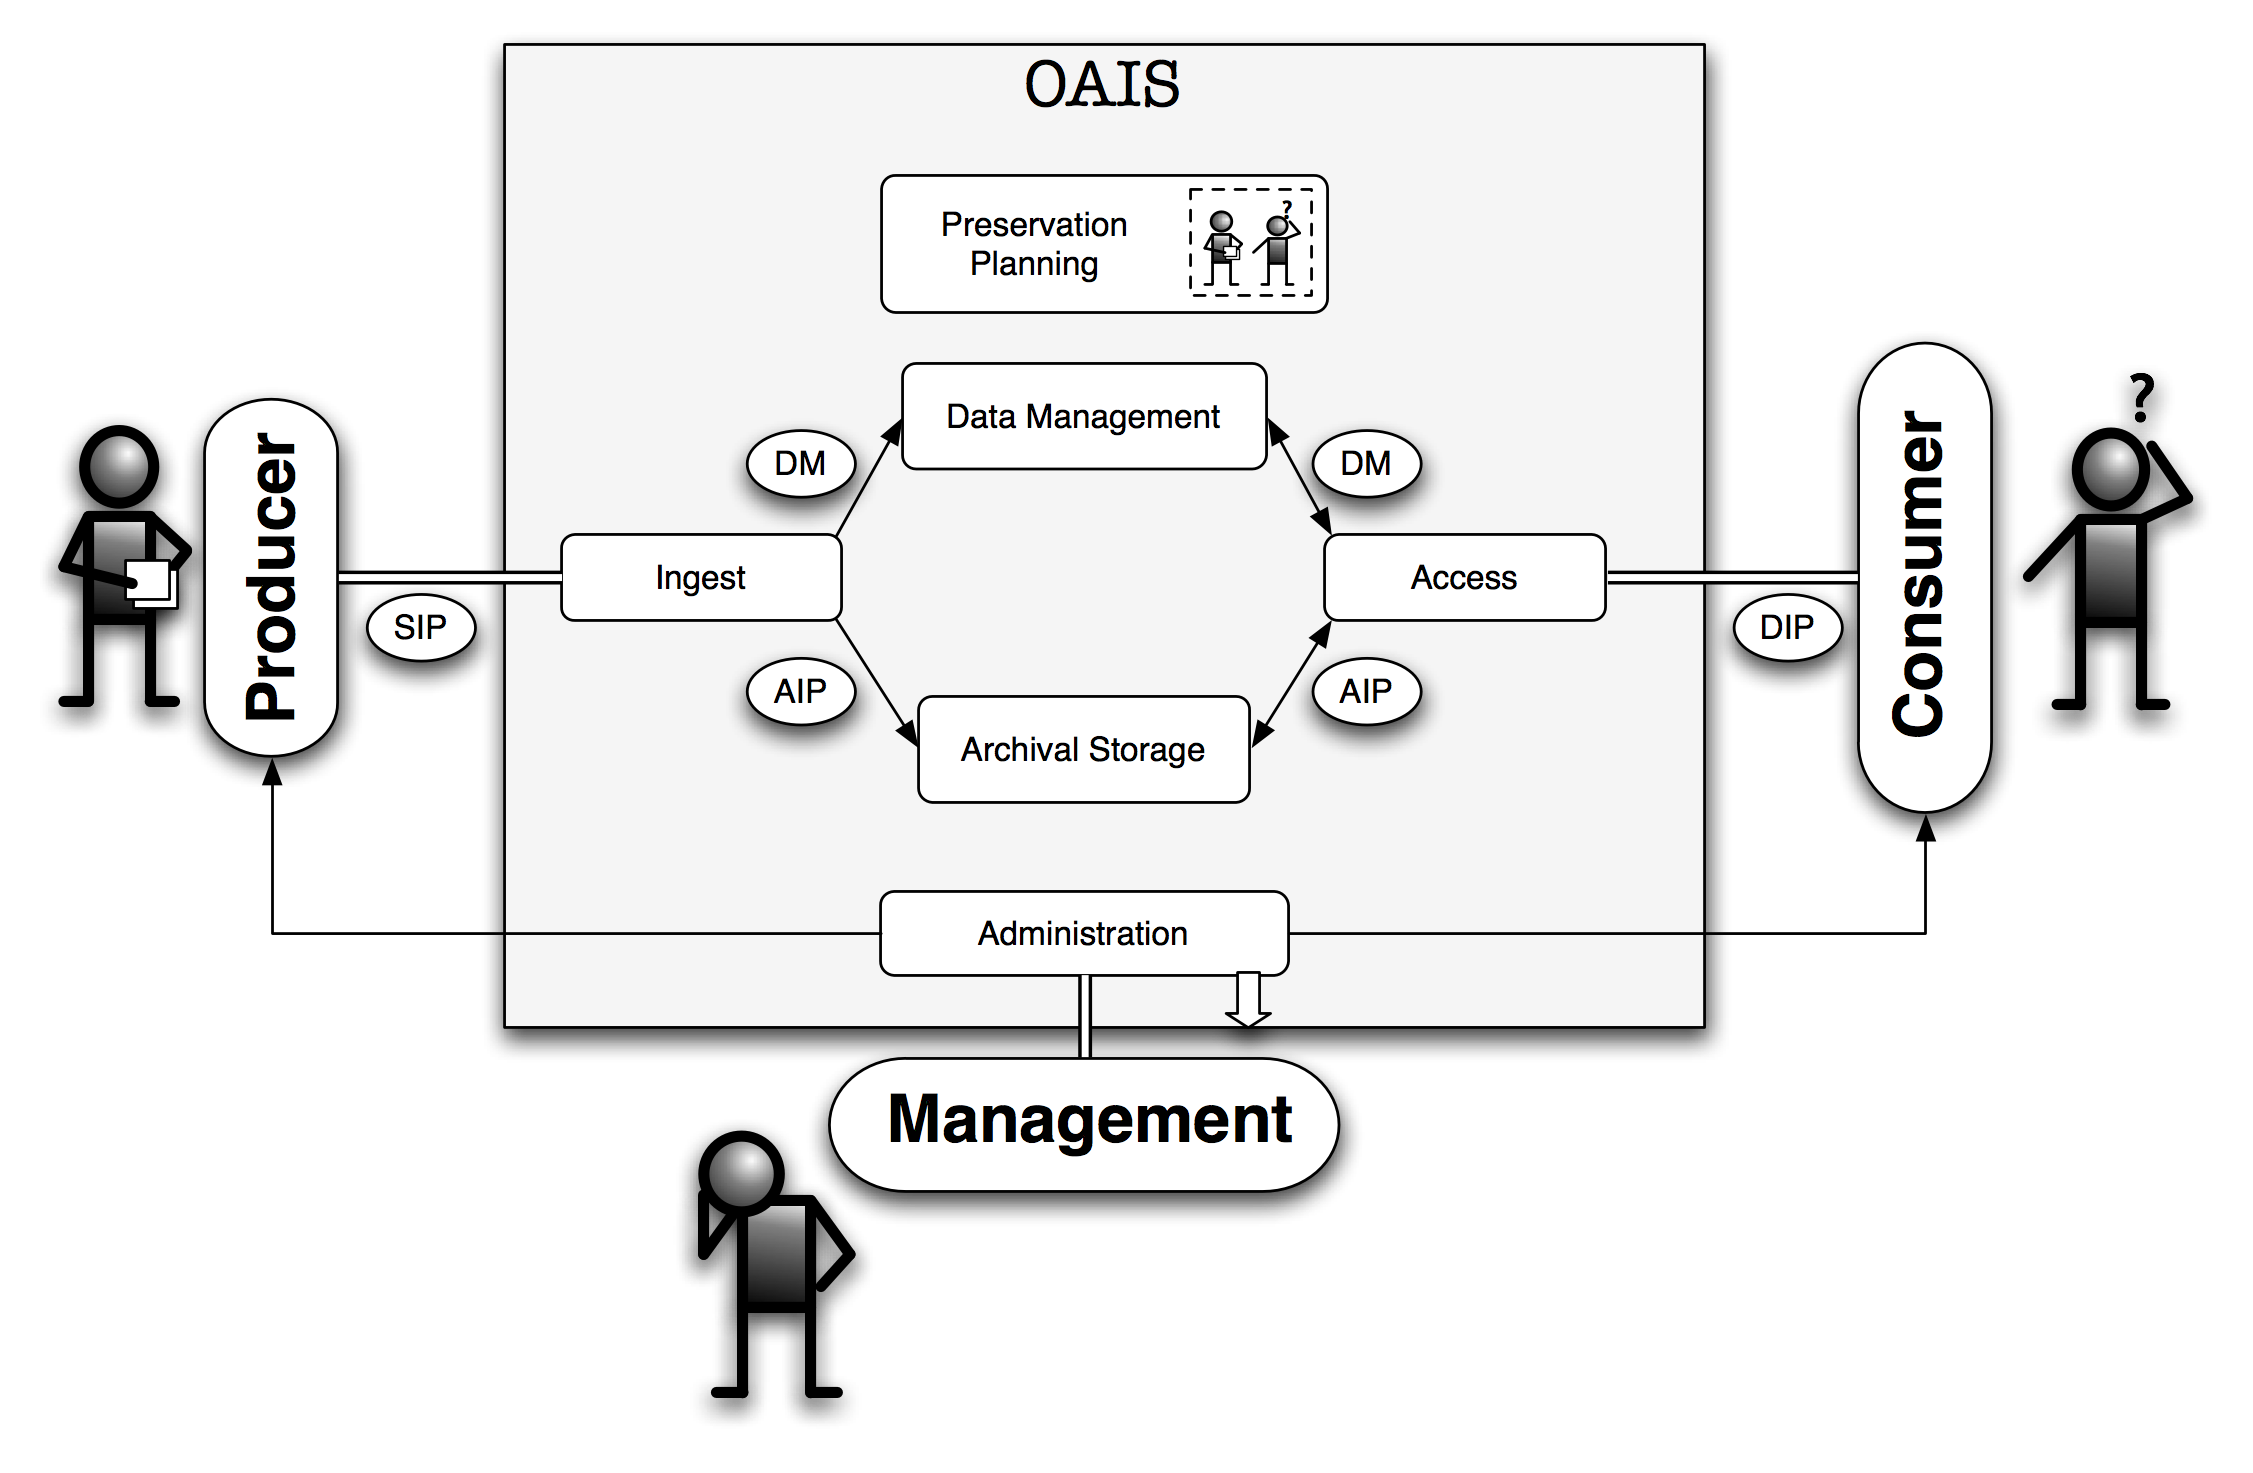
\includegraphics[width=1\textwidth,center]{images/arquitetura/oais}
  \caption{Modelo OAIS}
  \label{fig:oais}
\end{figure}

Como representado na Figura ~\ref{fig:oais}, o sistema irá interagir com três tipos distintos de atores:
\begin{description}[labelindent=1cm]
  \item[Produtores] que serão representados pelos Alunos.
  \item[Administrador] que serão representados pelos Docentes.
  \item[Consumidor] que serão representados pelos Utilizadores não Registados.
\end{description}
E será constituido por três mega processos:
\begin{description}[labelindent=1cm]
  \item[Ingestão] responsável pela receção e depósito de projetos.
  \item[Administração] responsável pela gestão interna do sistema.
  \item[Disseminação] responsável pela disseminação, distribuição e publicação dos objetos arquivados.
\end{description}

\subsection{Fluxo do Sistema}

Com o objetivo de perceber e organizar melhor o fluxo do nosso sistema, construimos um \textbf{Diagrama de Atividade} que de uma forma pouco pormenorizada demonstra sequencialmente as principais ações dos utilizadores do sistema. De notar que este diagrama será importante para perceber a ligação entre os vários utilizadores e as ações dependentes entre estes.

Com o \textbf{Diagrama de Atividade} da Figura ~\ref{fig:diagrama-blocos}, podemos consultar de forma simplificada o fluxo do nosso sistema.

\begin{figure}[H] 
  \centering
  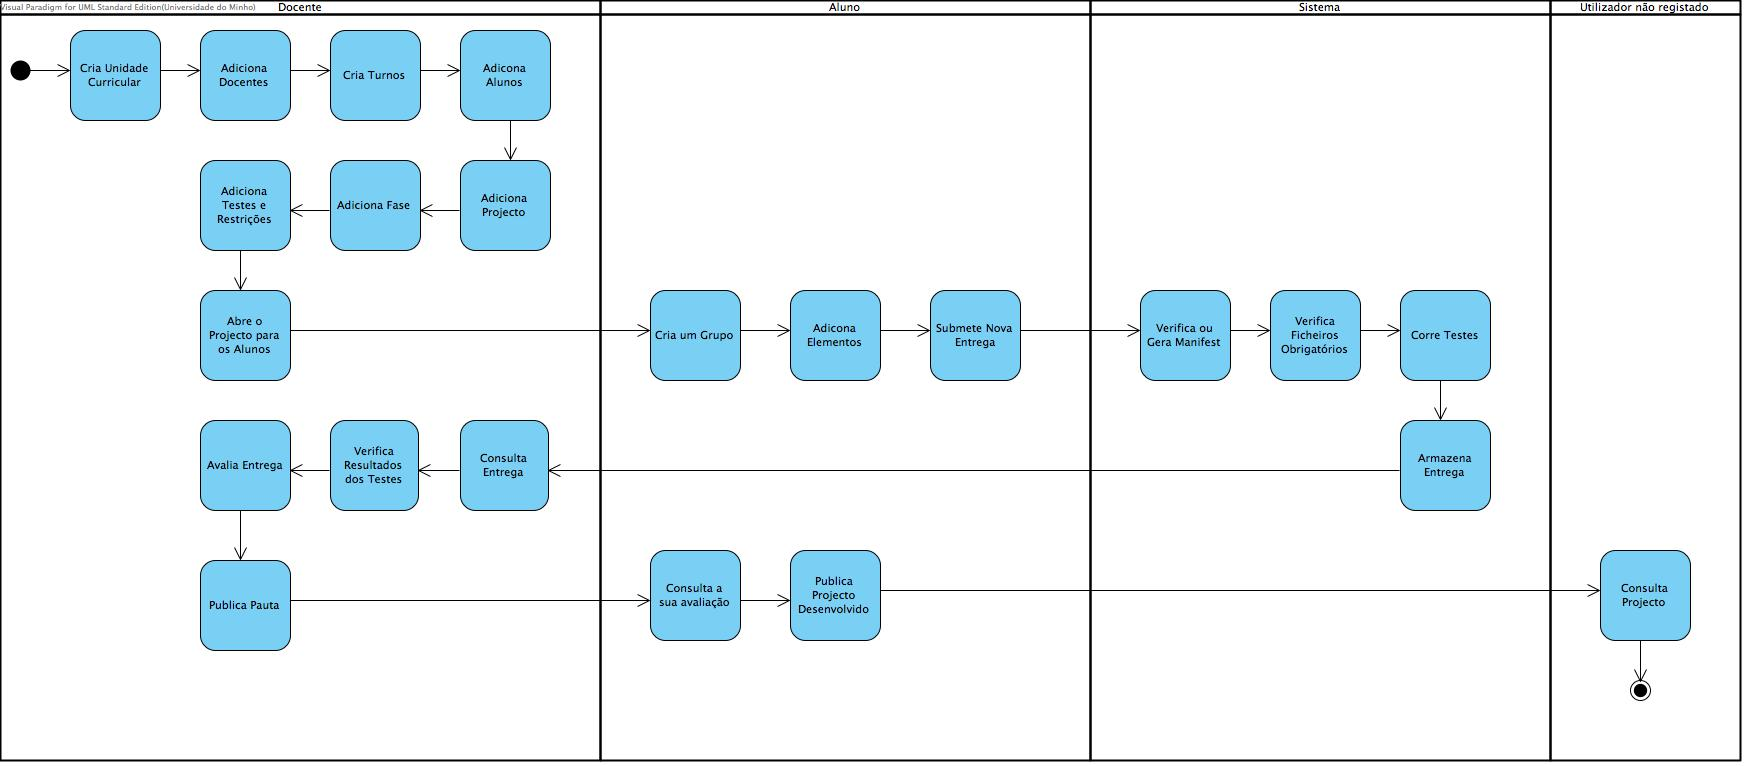
\includegraphics[width=1\textwidth,center]{images/arquitetura/diagrama-blocos}
  \caption{Fluxo do Sistema}
  \label{fig:diagrama-blocos}
\end{figure}

Para a representação do fluxo das funcionalidades mais complexas da aplicação, construiu-se \textbf{Diagramas de Atividade} que permitem representar essas mesmas funcionalidades mais pormenorizadamente.
Estes diagramas para além de ajudarem a perceber melhor o funcionamento do sistema nas tarefas mais relevantes, serão um excelente apoio na implementação do sistema.

Na Figura ~\ref{fig:criacao-projecto} podemos consultar o fluxo de criação de um projeto, desde o acesso ao sistema por parte de um docente, até ao acesso à página do projeto por parte de um aluno.

\begin{figure}[H] 
  \centering
  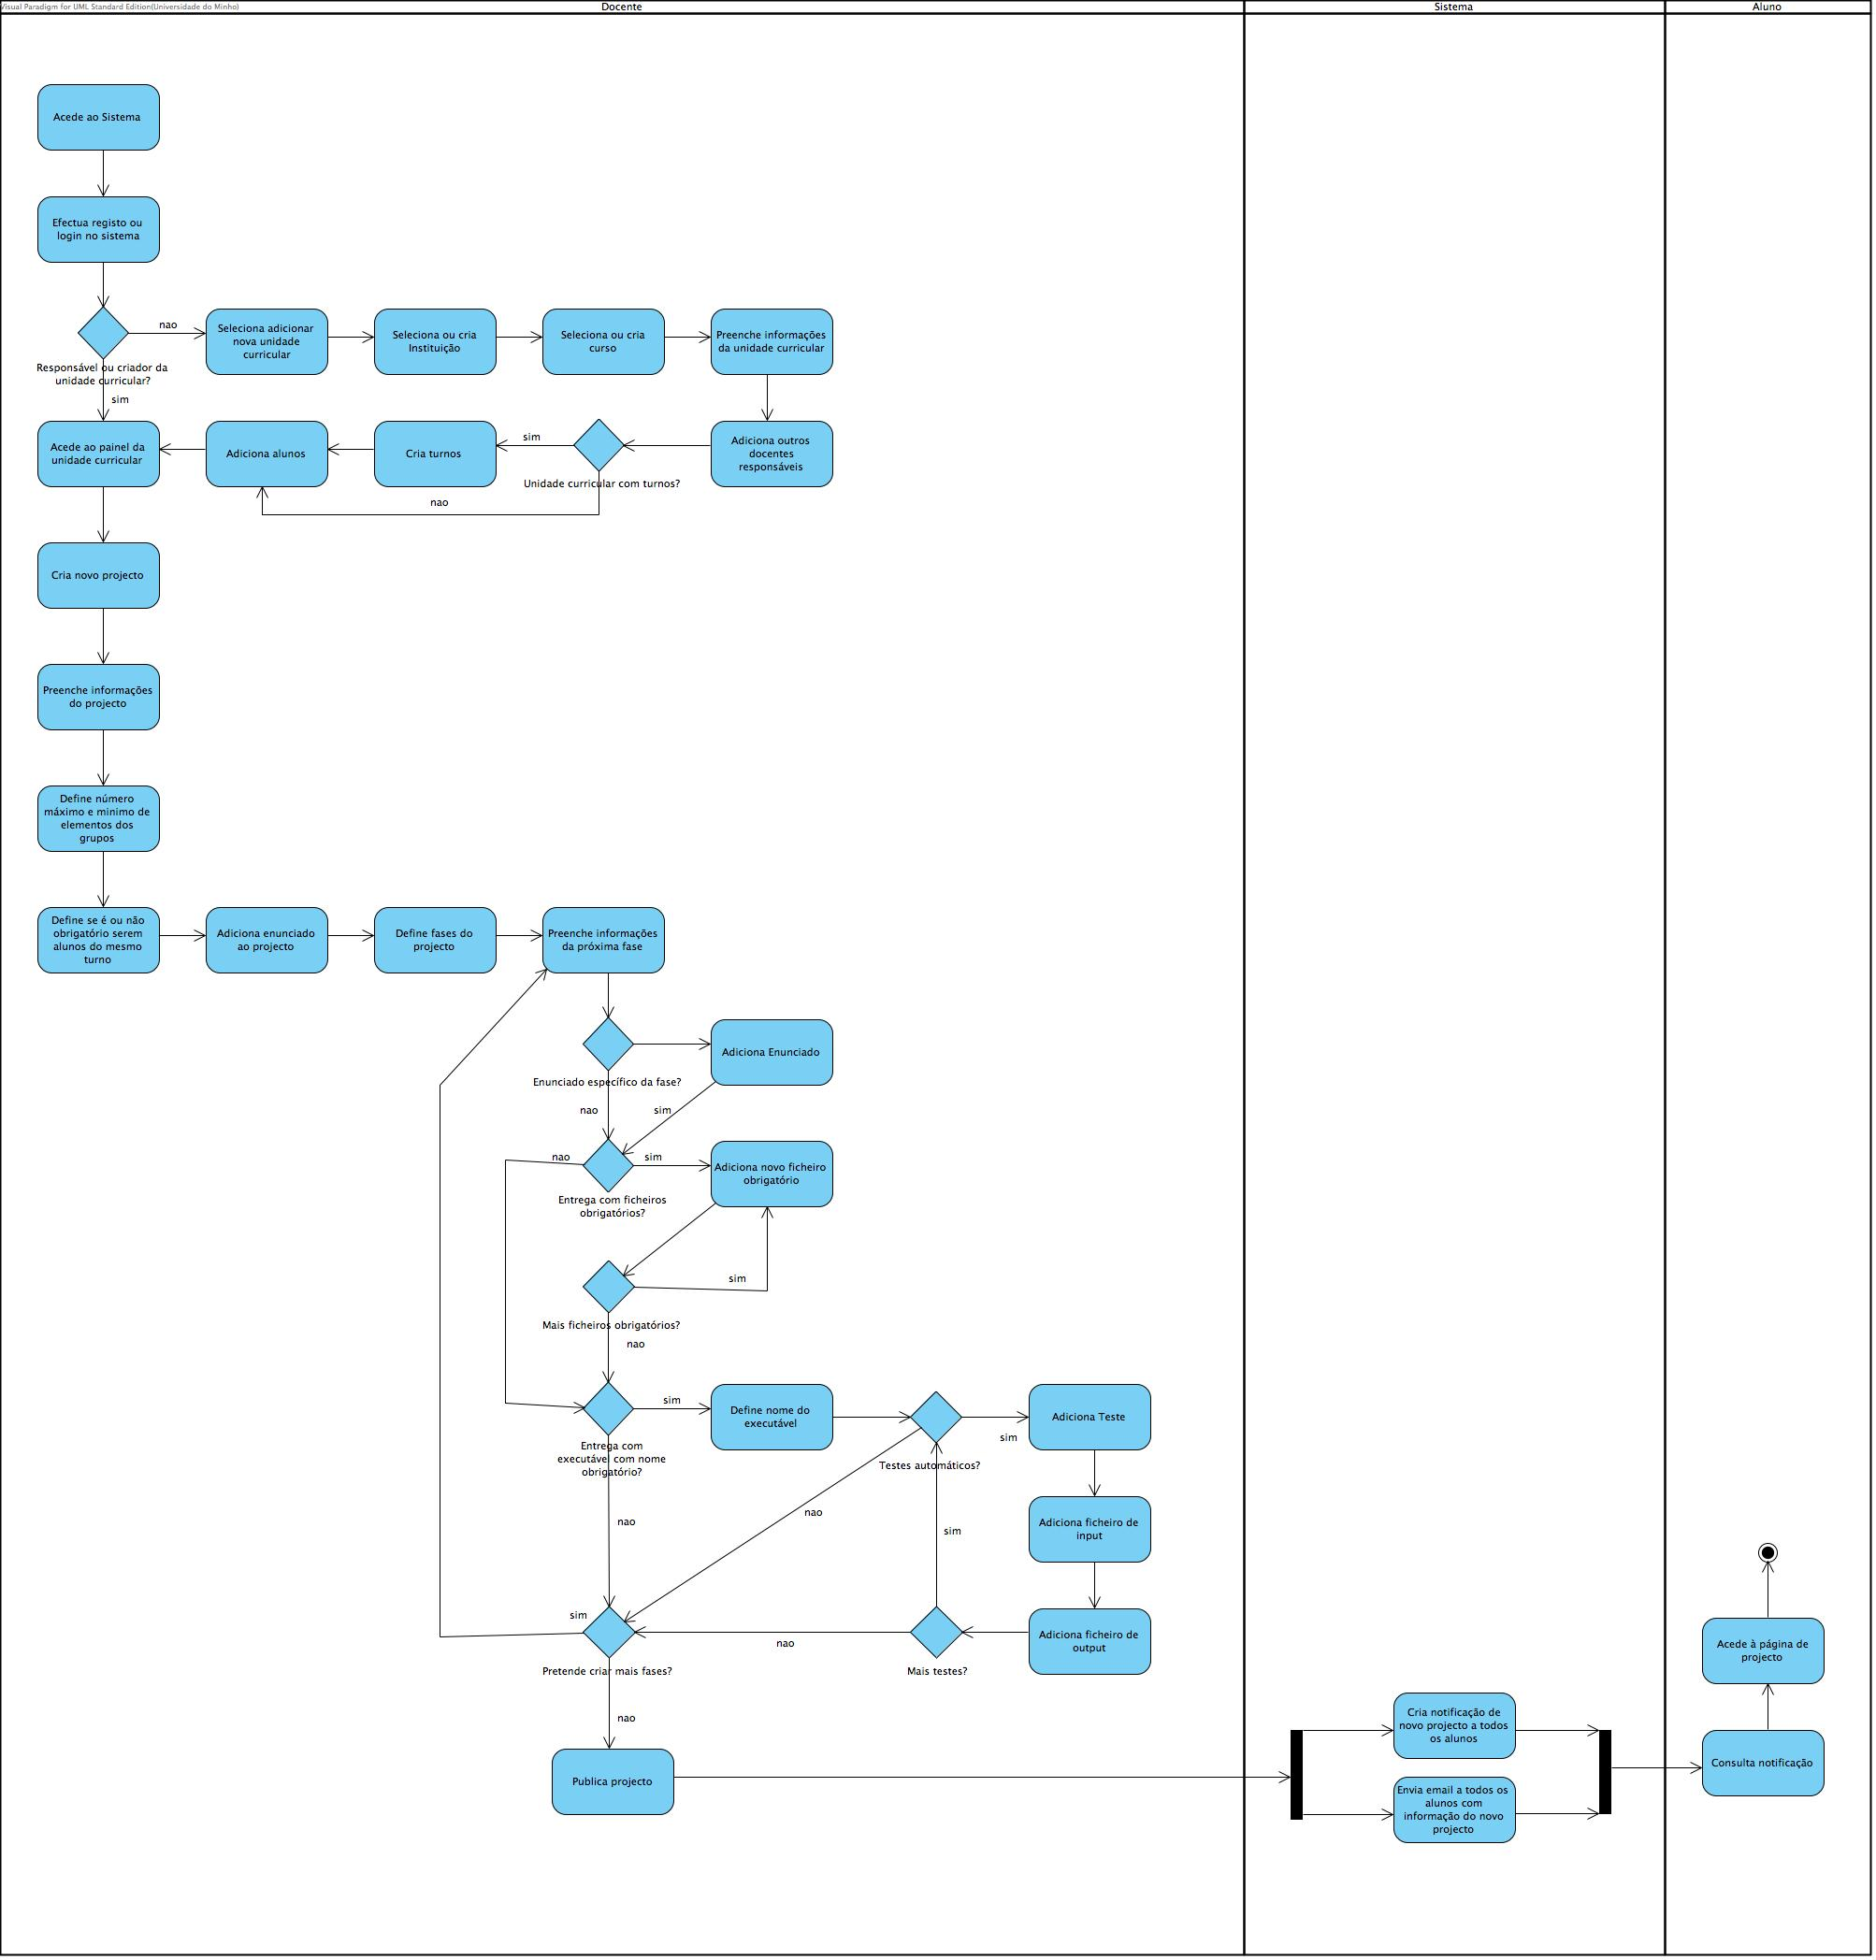
\includegraphics[width=1\textwidth,center]{images/arquitetura/criacao-projecto}
  \caption{Fluxo: Criar Projecto}
  \label{fig:criacao-projecto}
\end{figure}

Na Figura ~\ref{fig:submissao-projecto} podemos consultar o fluxo de submissão de um projeto, desde o acesso à página de um projeto por parte de um utilizador até à consulta das informações da entrega por parte de um docente.

\begin{figure}[H] 
  \centering
  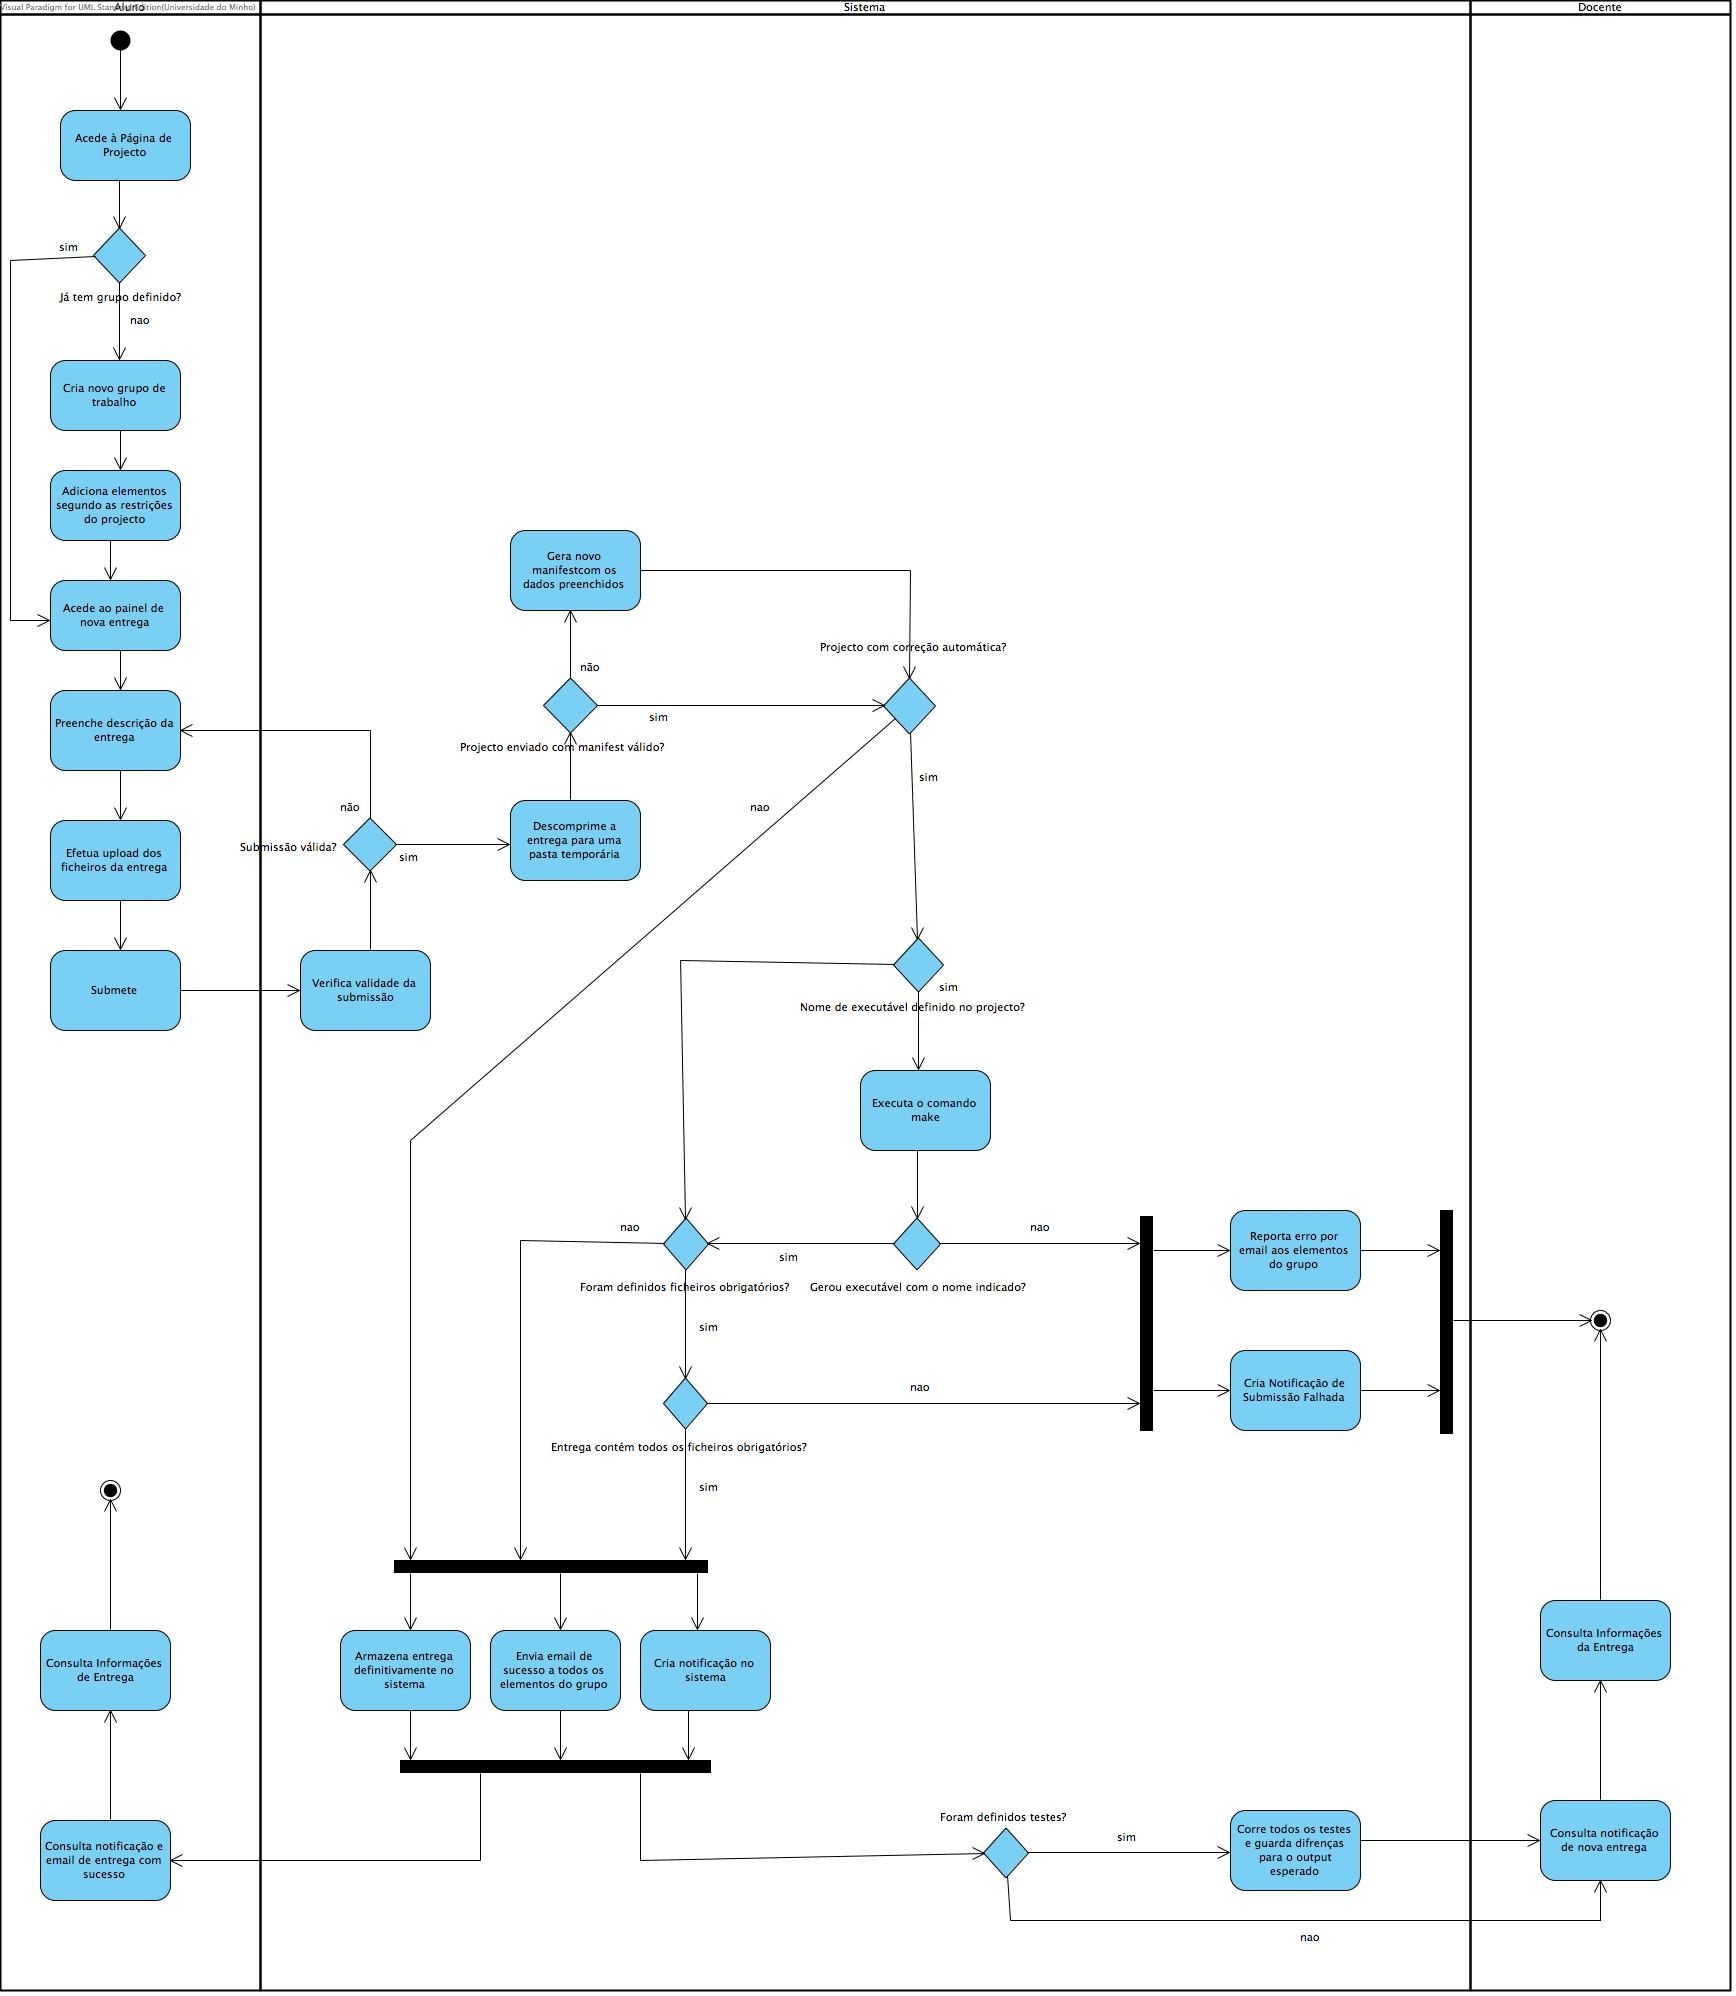
\includegraphics[width=1\textwidth,center]{images/arquitetura/submissao-projecto}
  \caption{Fluxo: Submeter Projeto}
  \label{fig:submissao-projecto}
\end{figure}

\section{Modelo de dados}

Uma das componentes importantes do desenho de um sistema de informação, passa por criar um modelo que explique as características de funcionamento e comportamento do \textit{software} a ser desenvolvido. A modulação para além de ajudar na compreensão do sistema, evita erros de programação, de projeto e de funcionamento.

\subsection{Modelo de Domínio}

Um dos primeiros passos na planificação do nosso sistema passou pela definição do \textbf{Modelo de Domínio}.
Podemos classificar como domínio do nosso sistema, o conjunto de características que descrevem a família de problemas que a nossa aplicação pretende solucionar.

Podemos consultar na Figura ~\ref{fig:modelo-dominio} os termos do nosso sistema e as relações existentes entre esses termos.

\begin{figure}[H] 
  \centering
  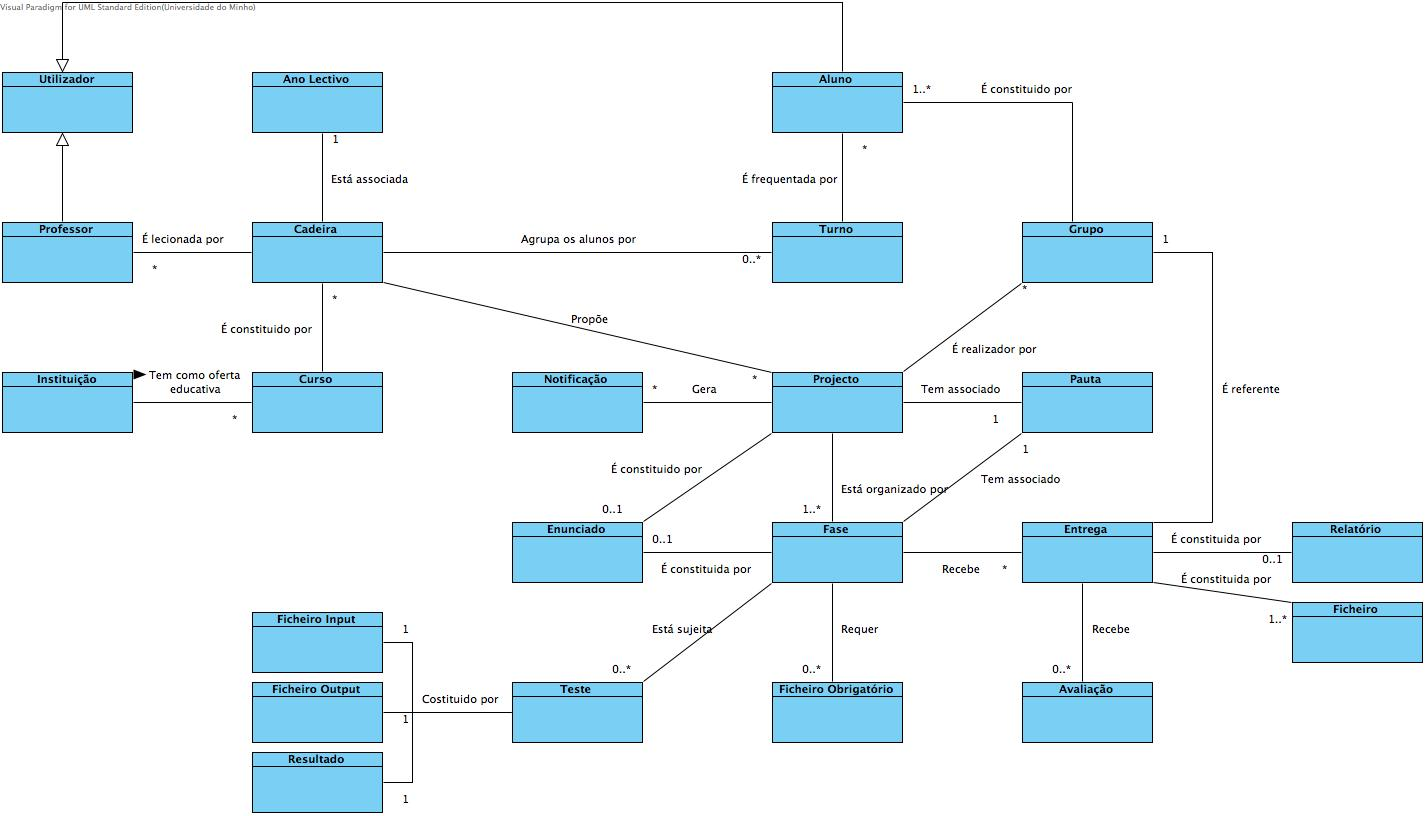
\includegraphics[width=1\textwidth,center]{images/modelo_dados/modelo-dominio}
  \caption{Modelo de domínio}
  \label{fig:modelo-dominio}
\end{figure}

\section{Repositório de informação}

Para a representação do repositório de informação do sistema, utilizar-se-á um \textbf{Diagrama entidade relacionamento}, que descreve o modelo de dados de um sistema com alto nível de abstração. 

Na Figura ~\ref{fig:der} pode-se consultar todas as tabelas que constituirão o sistema, assim como os seus atributos. De notar que os tipos especificados para os atributos podem não retratar corretamente os tipos que serão utilizados. Como se irá utilizar a \textit{framework} Ruby on Rails para desenvolvimento, esta permite uma maior abstração em relação aos tipos dos atributos da base de dados. Assim sendo os tipos serão definidos segundo o Diagrama de Classes apresentado anteriormente e a \textit{framework} fará a conversão automática conforme a base de dados que estivermos a utilizar.

\begin{figure}[H] 
  \centering
  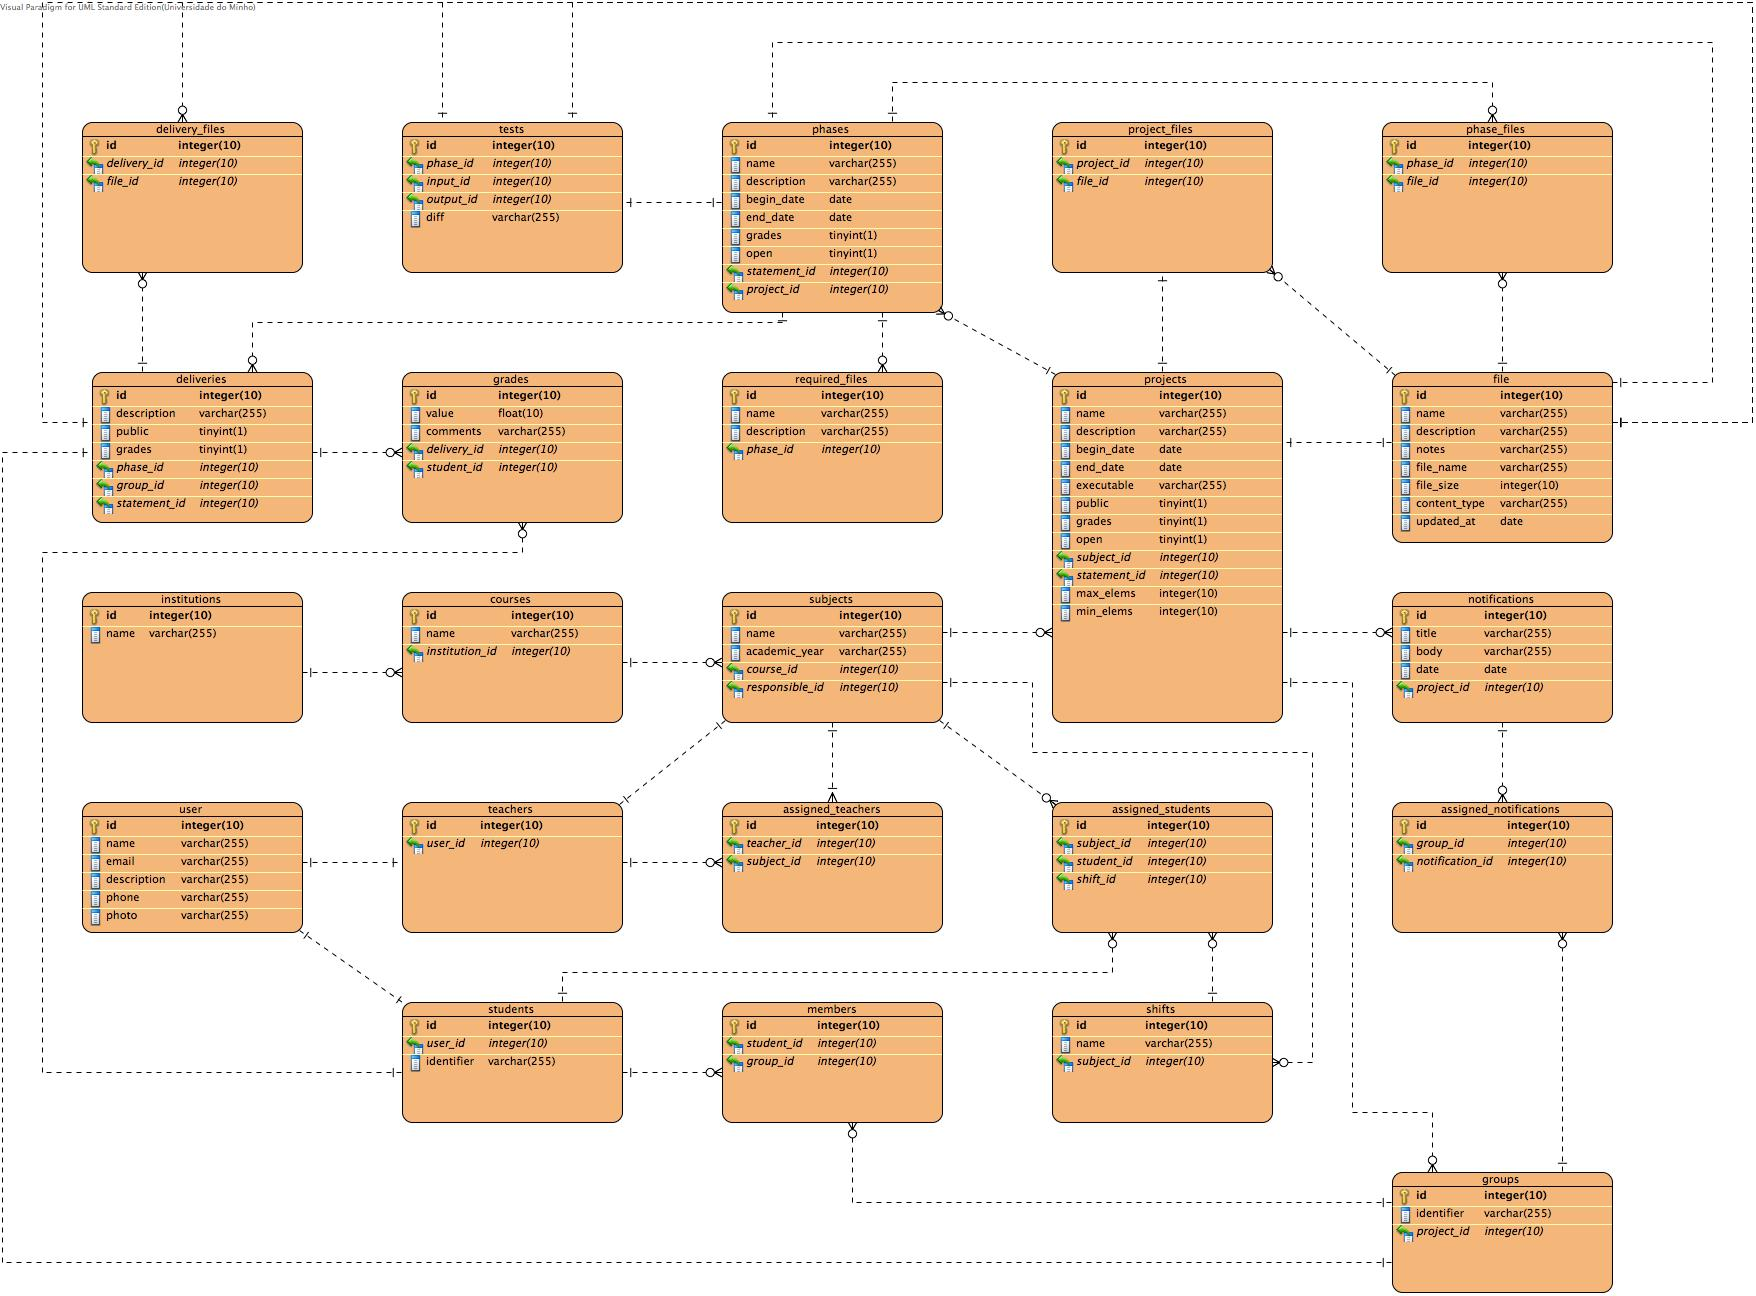
\includegraphics[width=1\textwidth,center]{images/repositorio_informacao/der}
  \caption{Diagrama Entidade Relacionamento}
  \label{fig:der}
\end{figure}

De notar que será utilizado \textbf{SQLite} em ambientes de desenvolvimento e testes, e \textbf{PostgreSQL} para ambientes de produção.

\section{Funcionalidades do sistema}

No que diz respeito às funcionalidades do sistema é necessário ter em conta a definição dos seus 
utilizadores e quais as objetivos que a aplicação se propõe a resolver.
Nesse sentido foram definidos três tipos de utilizadores cada um com um conjunto concreto de 
funcionalidades que lhes são fornecidas.
De forma a conseguir fazer este tipo de especificação foram idealizados os seguinte tipos de utilizadores
que interagirão com o sistema, sendo eles: utilizador não registado e utilizador registado na forma de 
docente e aluno.

\begin{figure}[htbp!] 
   \centering
   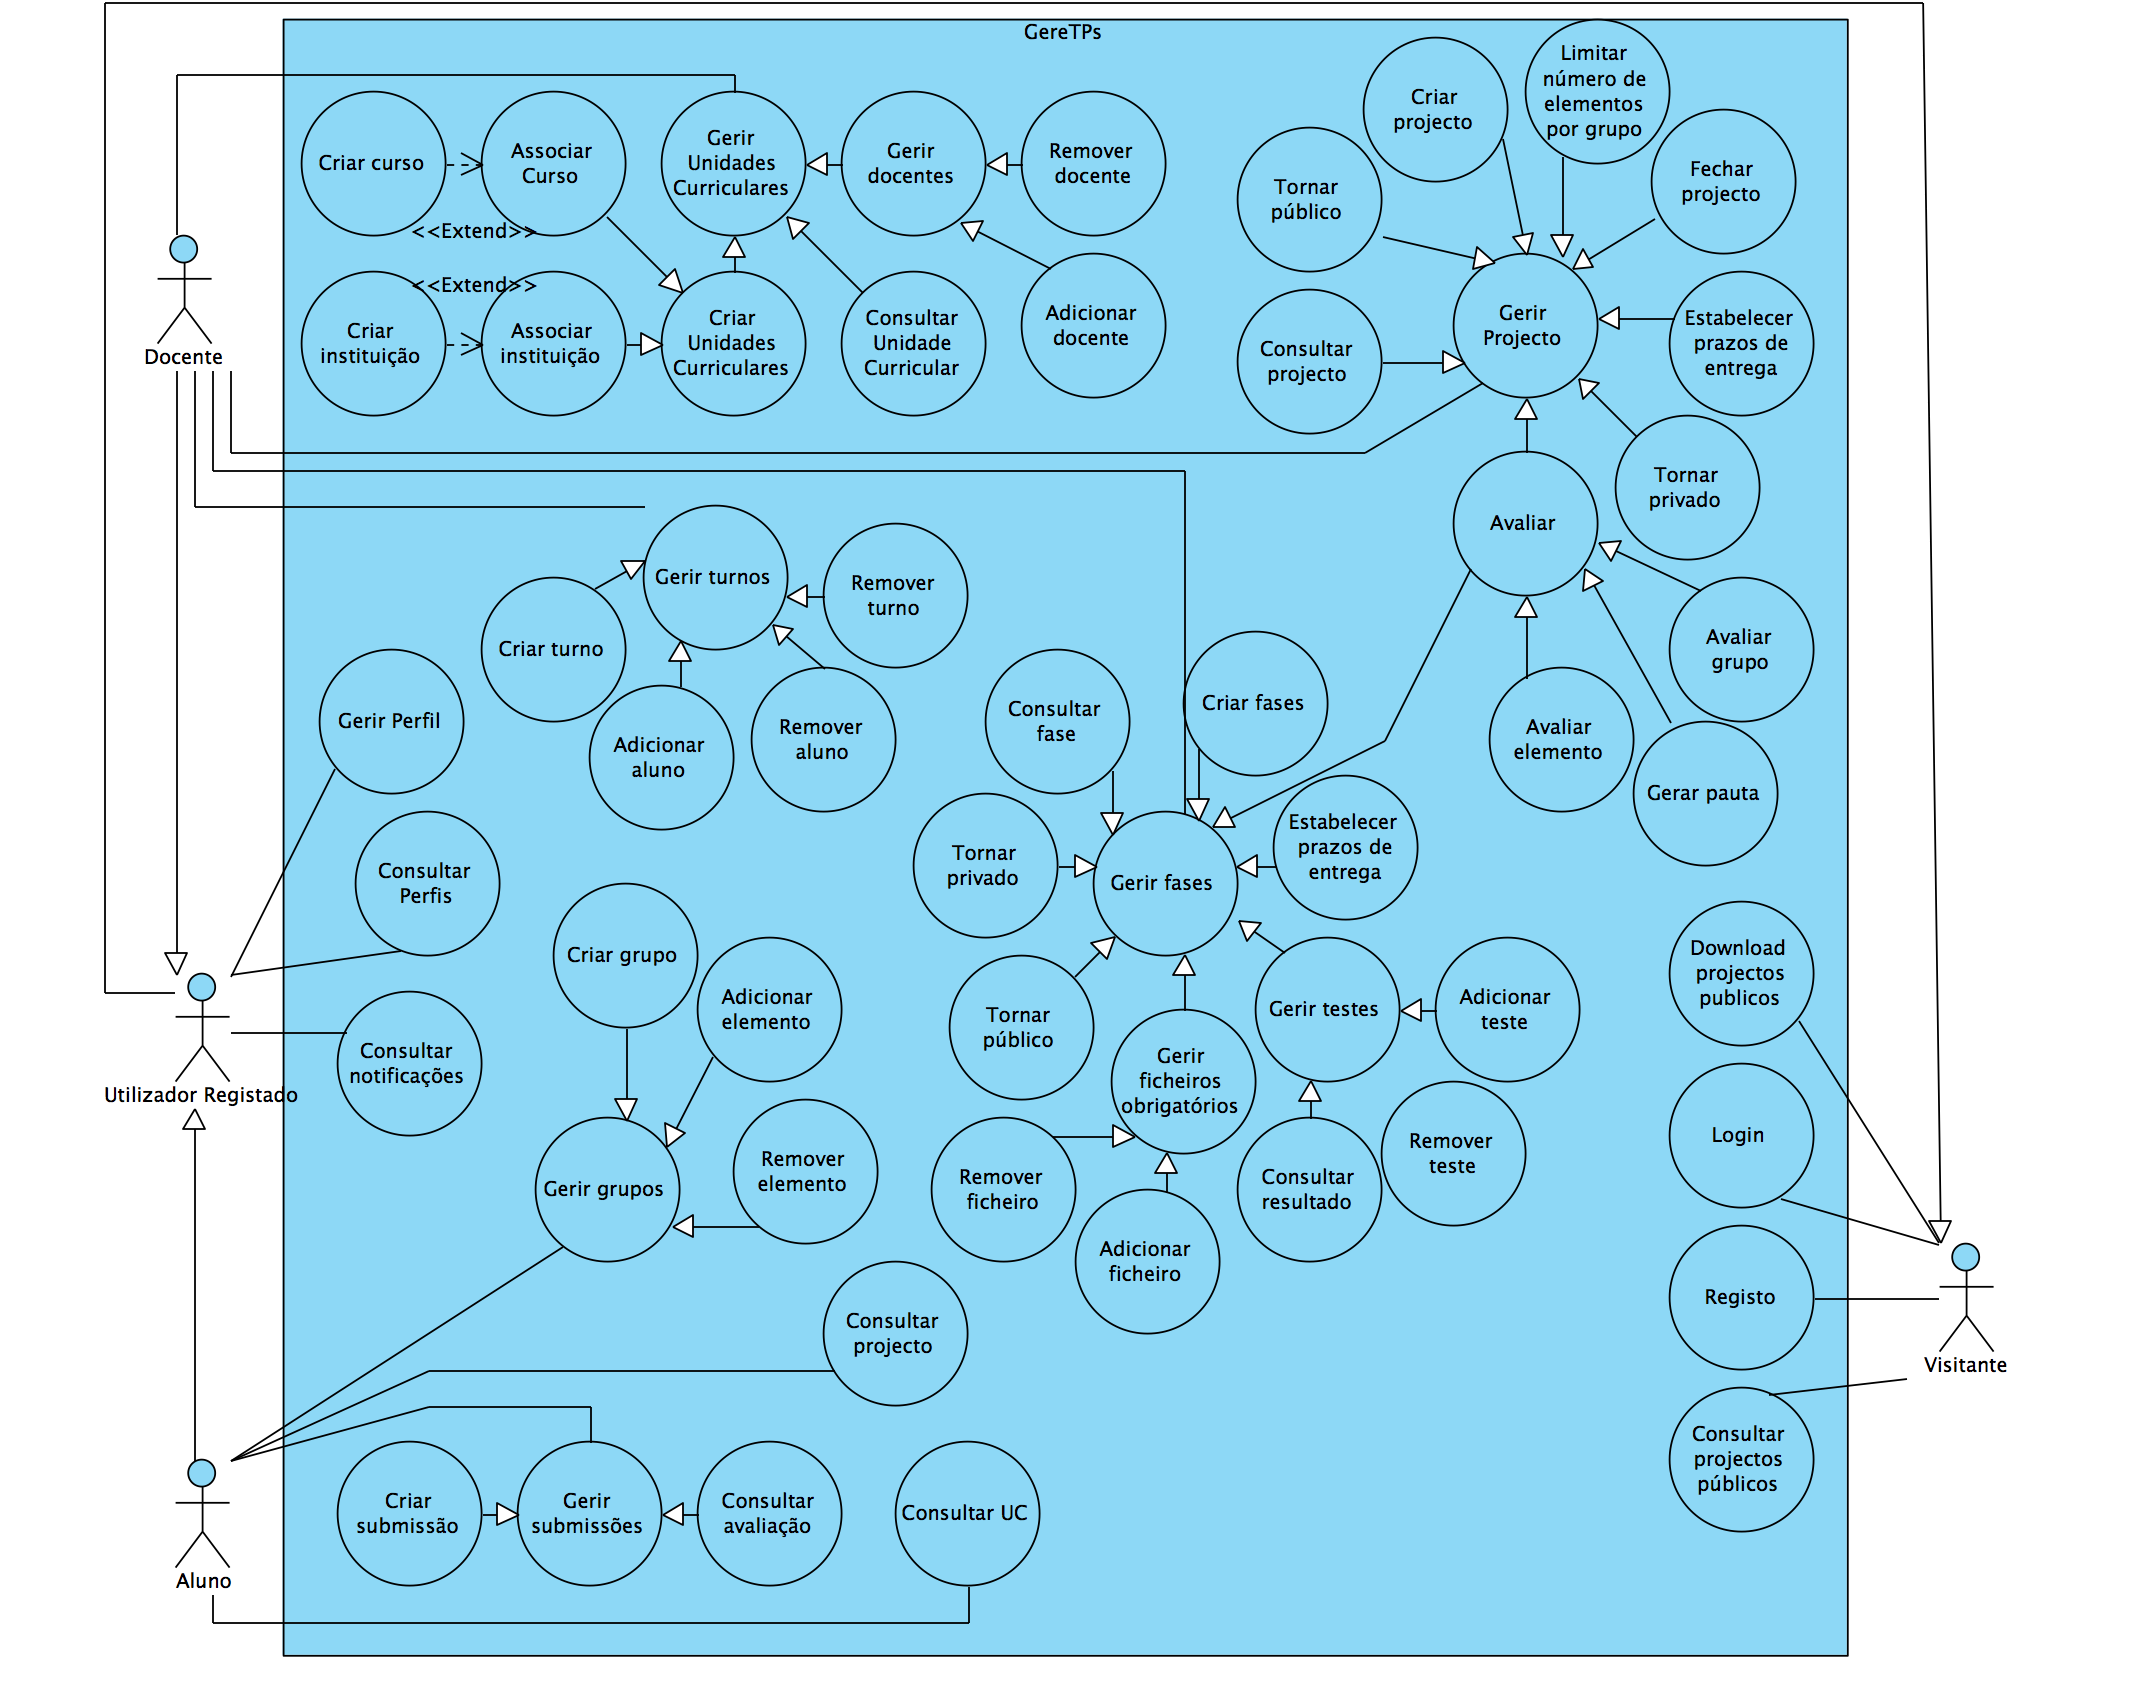
\includegraphics[width=1\textwidth]{images/funcionalidades/usecases.png}
    \caption{Diagrama com casos de uso dos utilizadores do sistema}
    \label{fig: usecases}
 \end{figure}

\subsection{Utilizadores não registados}

Como é possível ver no diagrama de Casos de uso representado na Figura \ref{fig: usecases}, no caso 
dos Utilizadores não registados, representados no diagrama pelo ator Visitante, são disponibilizadas
funcionalidades de registo, entrada no sistema, consulta e \textit{download} de projetos públicos.

Assim sendo é permitido a este tipo de utilizadores registarem-se na aplicação, providenciando informações
pessoais e criando então uma conta persistente com os seus dados, definindo-se a si próprio como
docente ou aluno. Após o registo é-lhes permitida a entrada no sistema com as credenciais de acesso
definidas aquando do registo prévio. Como utilizadores não registados podem também consultar e procurar
todos os projetos disponibilizados por outros utilizadores na aplicação, assim como também lhes é fornecida
a opção de descarregarem os mesmos projetos para o dispositivo de onde acessam.

\subsection{Docentes}

O seguinte tipo de utilizadores descrevem-se como utilizadores registados, sendo-lhes 
disponibilizadas funcionalidades específicas dentro do ambiente da aplicação. Nesse sentido, para 
além de serem uma extensão de Utilizadores não registados após o registo, são-lhes conferidas um
grupo de funcionalidades adicionais que descrevem o comportamento deste tipo de utilizador.

A um docente são disponibilizados quatro grupos de funcionalidades, como é possível observar na Figura
\ref{fig: usecases}. Esses grupos de funcionalidades são a gestão de unidades curriculares, turnos, 
projetos e fases.

No que diz respeito à gestão de unidades curriculares é tornado possível a este tipo 
de utilizador vários tipos de ações sobre as mesmas, nomeadamente, a consulta, a criação e 
remoção, a gestão de docentes, atualização das informações associadas, entre 
outras.

Para além disso, dentro de uma unidade curricular também é possível proceder-se 
à gestão de turnos. Nesse aspeto, é providenciado ao docentes tarefas como consulta, 
criação e remoção de turnos bem como a adição e remoção de alunos desses mesmo 
turnos.

Relativamente à gestão dos projetos de uma unidade curricular são fornecidas 
aos docentes as ferramentas para a consulta, criação e remoção, publicação, 
estabelecimentos de prazos assim como limitações ao número de elementos de um 
grupo, avaliação de um elemento ou grupo e por fim para geração de pautas, de 
todos os projetos associados a uma unidade curricular onde o docente seja 
responsável.

Por fim, a gestão de fases de um projeto é definida por funcionalidades como a 
sua criação e remoção, consulta, tipo de visibilidade, definição de 
obrigatoriedade de ficheiros, definição de testes sobre entregas e estabelecimento de prazos limite 
para submissões.

\subsection{Alunos}

Tal como o tipo de utilizador Docente, o tipo de utilizador Aluno é uma extensão 
de um utilizador não registado após o registo. Este tipo de utilizador é 
definido pelas funcionalidades que lhe são disponibilizadas pelo sistema. Dentro 
destas funcionalidades podemos destacar um conjunto delas, nomeadamente a 
consulta de projetos e unidades curriculares, a gestão de grupos e de submissões de projetos.

No que diz respeito à gestão de grupos é possível um aluno criar um grupo dentro 
de um projeto e adicionar e remover outros alunos como elementos do grupo.

Para além disso também são disponibilizadas ferramentas na aplicação que permite 
aos alunos fazerem submissões ou entregas de projetos dentro de uma unidade 
curricular de onde façam parte de um dos turnos. Para além disso também lhes é 
possível consultar as avaliações dadas pelos docentes às suas submissões assim 
como consultar a unidade curricular e as pautas da mesma.

\newpage
\section{Protótipos para a interface da aplicação}
 \subsection{Primeiros protótipos}

Durante a produção dos primeiros protótipos, teve-se como objetivo identificar de que formas as várias funcionalidades do sistemas iriam estar presentes na aplicação, sem haver preocupações com questões estéticas.Este protótipos são fundamentais, uma vez que demonstrem alguns dos cenários mais complexos e ajuda a compreensão de fluxos ou processos.
Este protótipos foram desenvolvidos usando a aplicação \href{http://balsamiq.com/products/mockups/}{\emph{Balsamiq Mockups}}(Figura ~\ref{fig: balsamiq}).\\

 \begin{figure}[htbp]
        \centering
        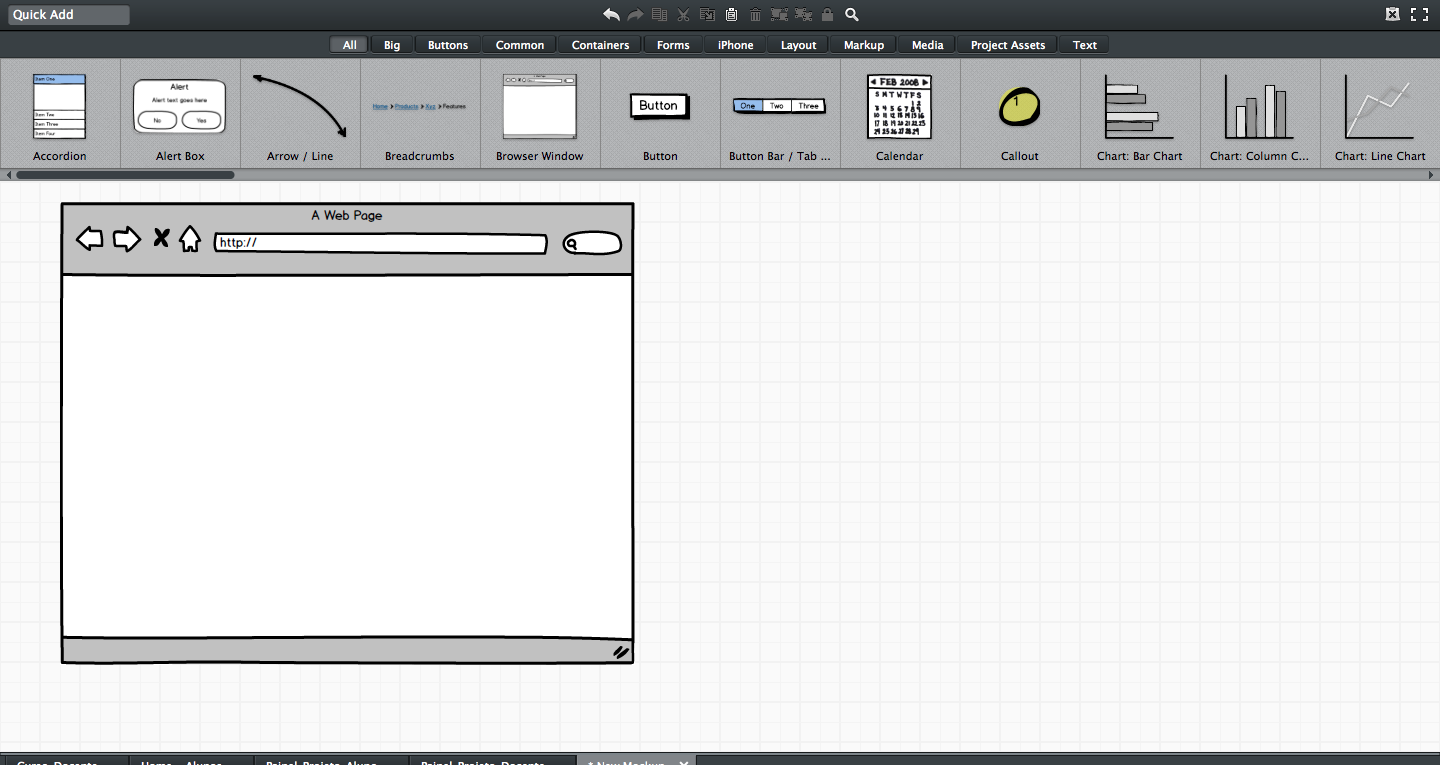
\includegraphics[width=1\textwidth]{images/prototipos/mockups/balsamiq.png}
         \caption{\emph{Balsamiq Mockups}}
         \label{fig: balsamiq}
\end{figure}

Sobre os protótipos desenvolvidos, teve-se como preocupação a simplicidade da página, a quantidade de informação e o tempo de navegação, isto é a quantidade de ações que um utilizador tem que fazer para passar de uma página para outra.\\
Começando pela página inicial (Figura ~\ref{fig: home}) está mostra as várias funcionalidades da aplicação, fazendo a distinção entre alunos e docentes.A partir da página inicial o utilizador pode fazer efetuar registo, login ou procura projetos públicos. \\

\begin{figure}[htbp]
        \centering
        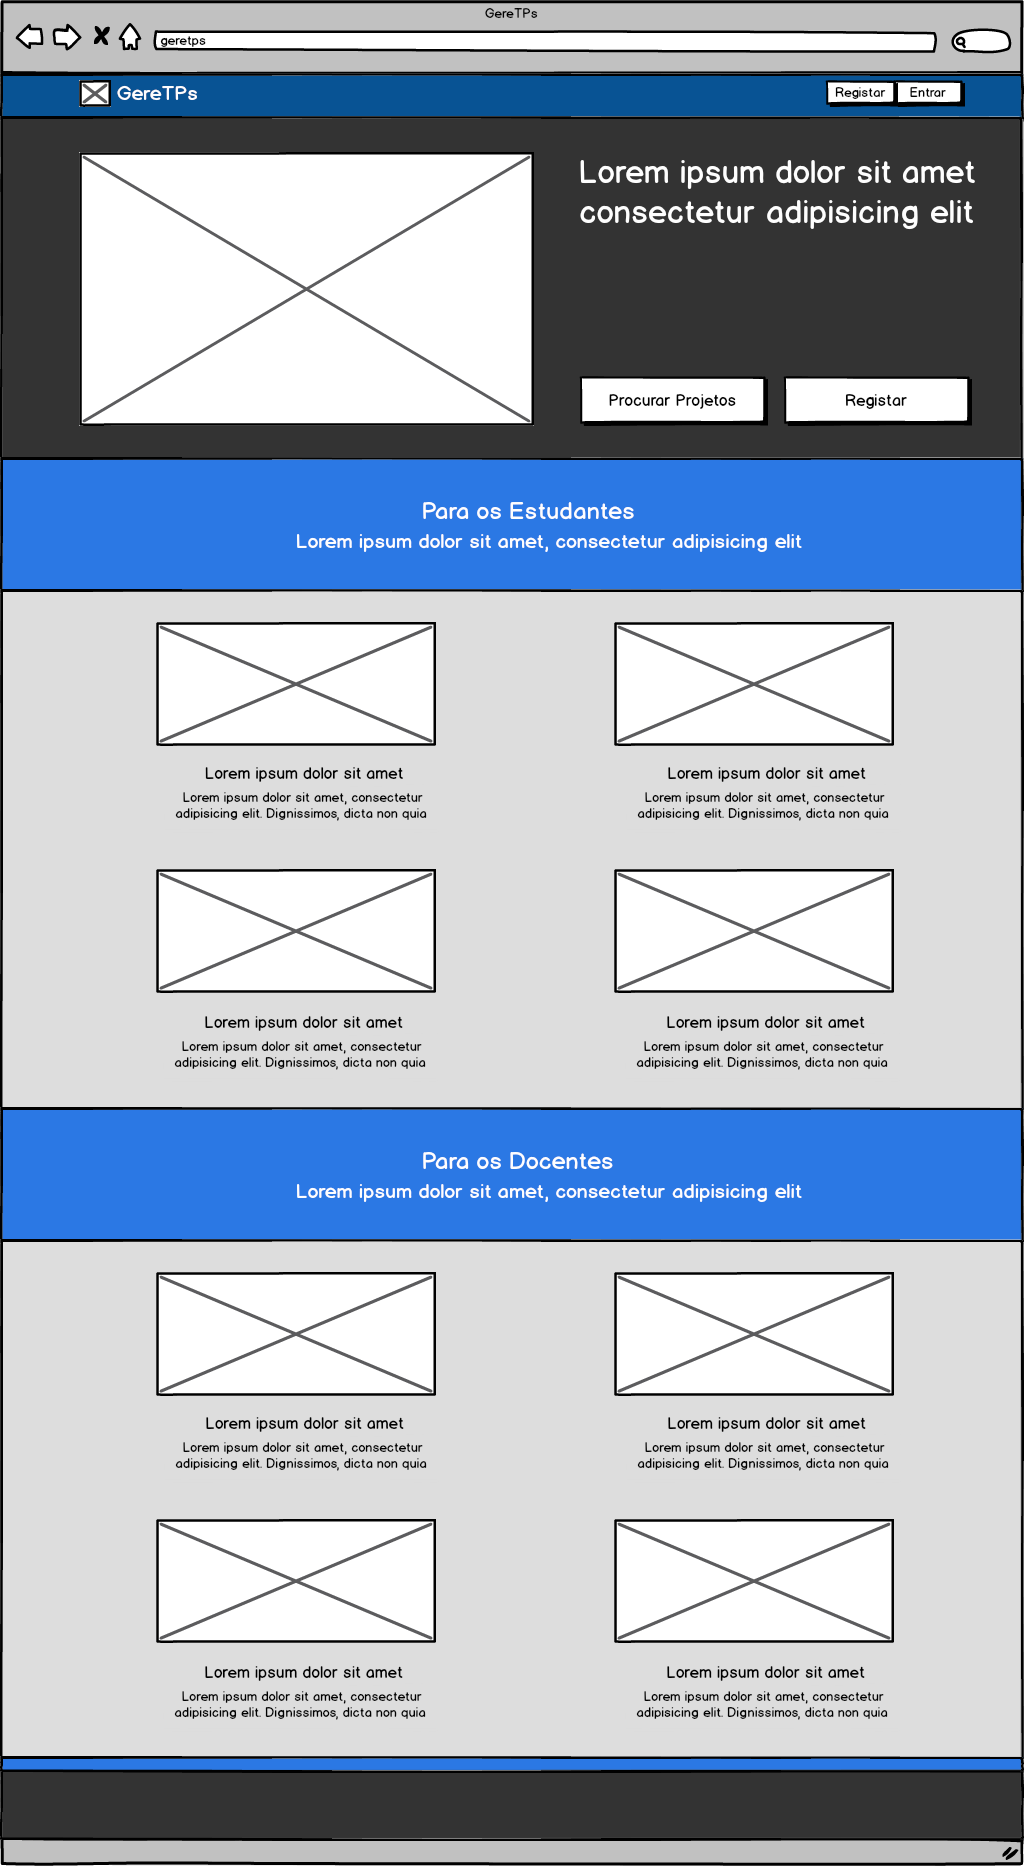
\includegraphics[width=1\textwidth]{images/prototipos/mockups/home.png}
         \caption{Página inicial}
         \label{fig: home}
\end{figure}

No painel de uma disciplina(Figura ~\ref{fig: cursodocente}), um docente pode ter acesso aos últimos acontecimentos dentro das disciplina, sabendo quando aconteceram submissões nos projetos desta, assim como alterações da mesma.Também existem informações sobre os projetos criados na disciplina, no qual são apresentadas informações sobre o nome do projeto, número de fases, estado e número de entregas até ao momento. Também é possível adicionar professores de forma direta sem que haja a necessidade de abrir formulários adicionais e fazer gestão de turnos. Caso contrário apenas poderá ver o estado dos turnos e quais são os docentes da disciplina.\\

\begin{figure}[htbp]
        \centering
        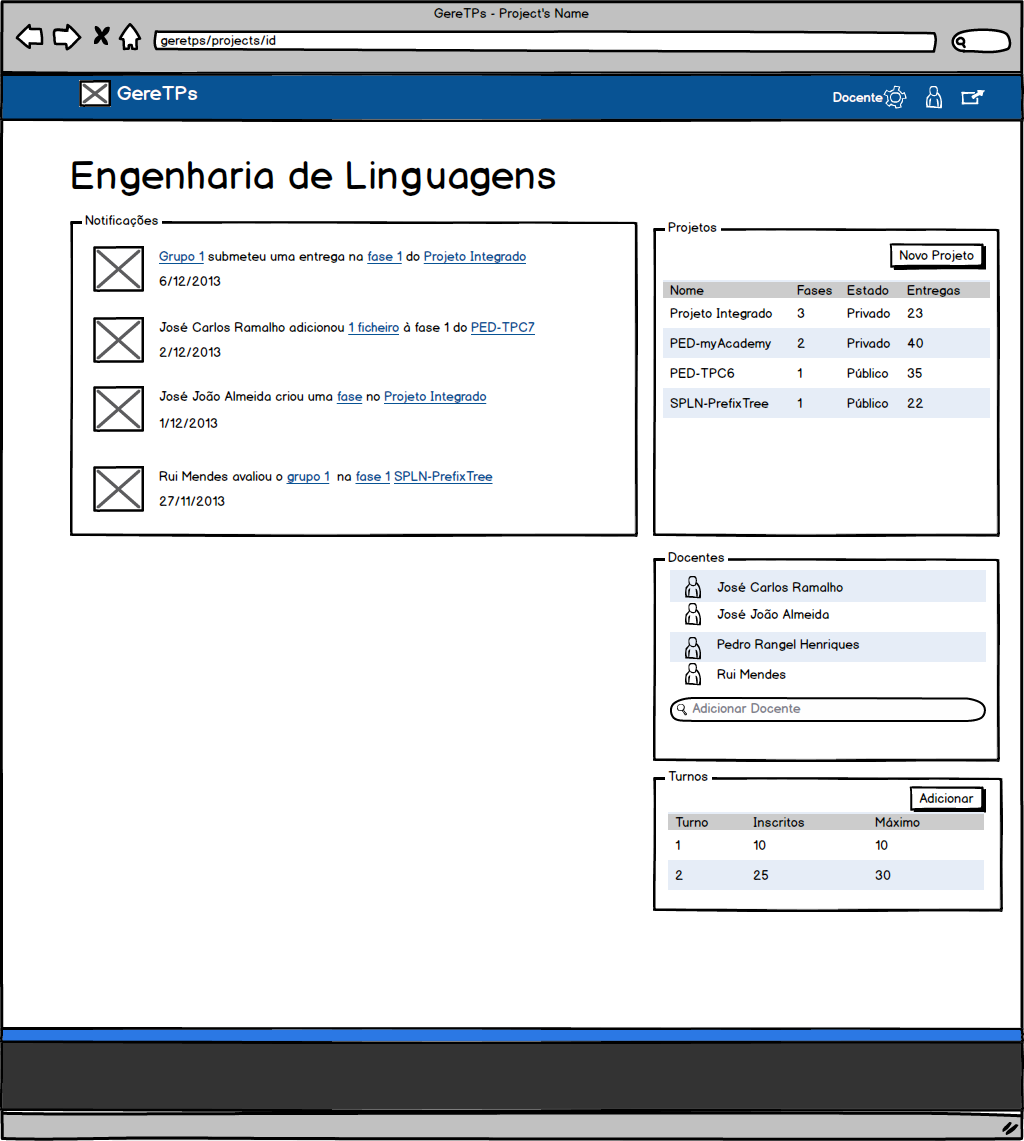
\includegraphics[width=1\textwidth]{images/prototipos/mockups/cursodocente.png}
         \caption{Painel de projeto de um aluno}
         \label{fig: cursodocente}
\end{figure}

Na painel de pesquisa de projetos(Figura ~\ref{fig: projetospublicos}), todos os utilizadores tem acesso aos projetos públicos. Nesta página o utilizador pode filtrar uma pesquisa de forma a que o processo seja mais rápido. Os resultados de uma pesquisa são apresentados sob forma de blocos, desta forma, garante-se um maior aproveitamento do espaço livre da página.\\

\begin{figure}[htbp]
        \centering
        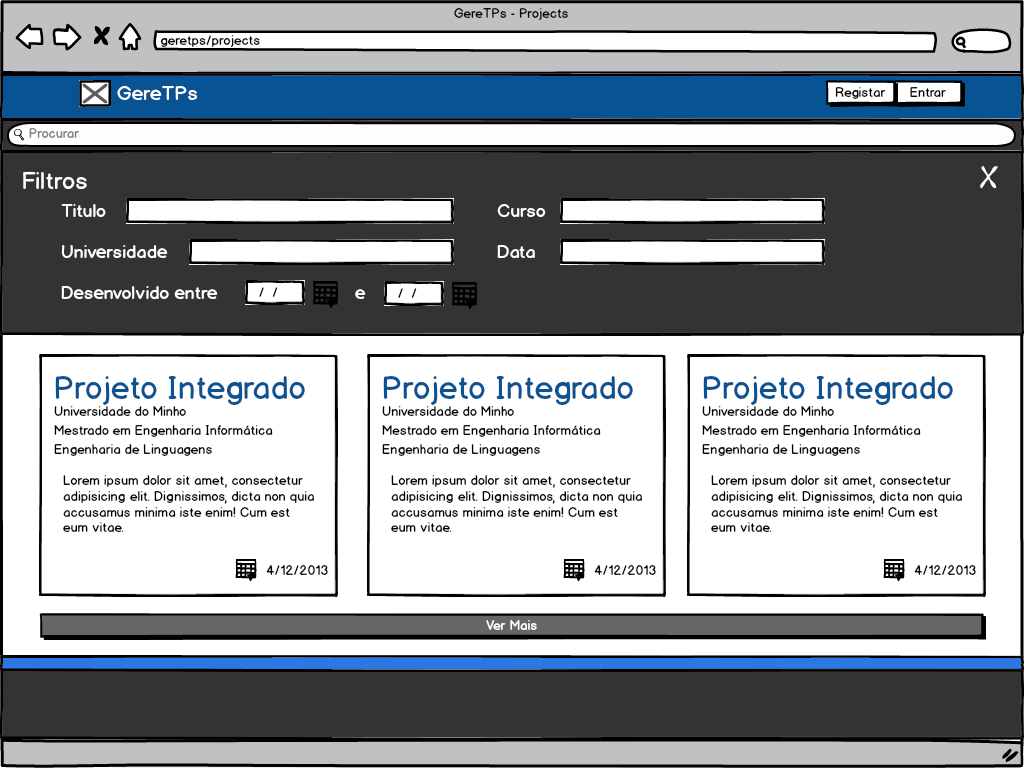
\includegraphics[width=1\textwidth]{images/prototipos/mockups/Projetos.png}
         \caption{Listagem dos projetos públicos}
         \label{fig: projetospublicos}
\end{figure}

Quando dentro do painel de um projeto, um docente pode:

\begin{itemize}
        \item Alterar informações do projeto
	\item Adicionar um enunciado, tal como outros ficheiros
	\item Gerir os grupos criados dentro do projeto
	\item Gerir as fases do projeto
	\item Consultar as submissões feitas até ao momento
        \item Adicionar/Remover testes
\end{itemize}
tal como se pode ver na Figura ~\ref{fig: painelprojetodocente}.\\

\begin{figure}[htbp]
        \centering
        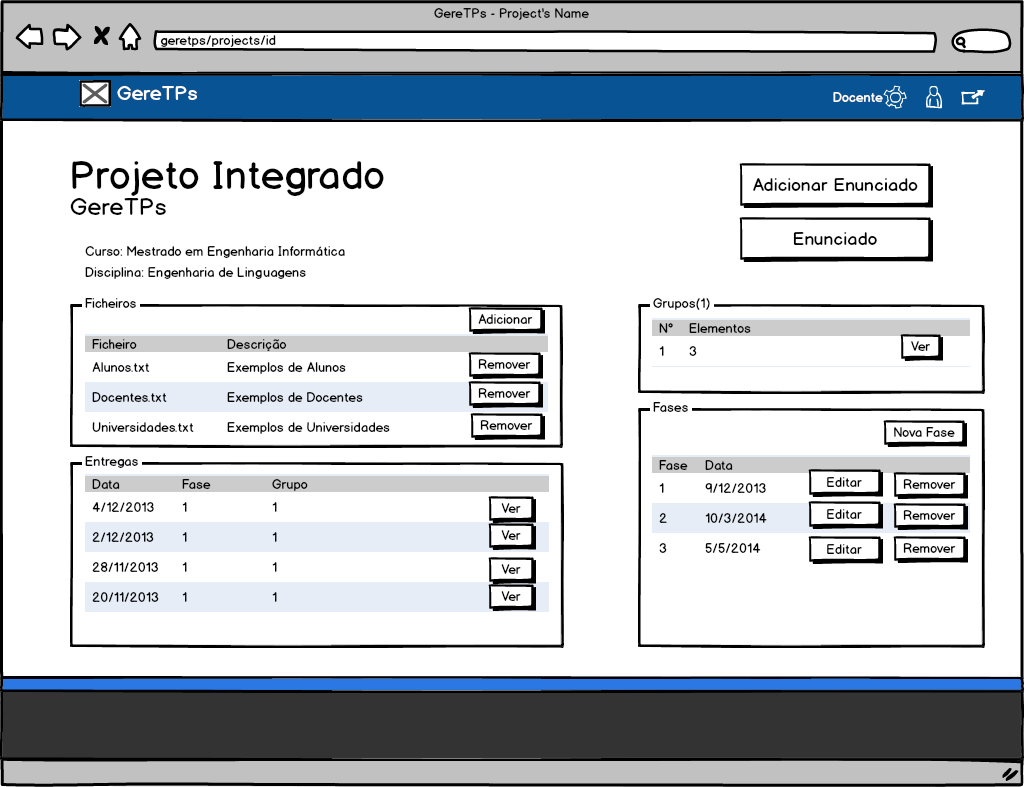
\includegraphics[width=1\textwidth]{images/prototipos/mockups/painelprojetodocente.png}
         \caption{Painel de projeto de um docente}
         \label{fig: painelprojetodocente}
\end{figure}

Um aluno pode consultar as informações dadas pelos os docente, consultar as entregas efetuadas pelo grupo, fazer a gestão do seu grupo e aceder a página de submissão de um projeto, como é possível ver na Figura ~\ref{fig: painelprojetoaluno}.\\

\begin{figure}[htbp]
        \centering
        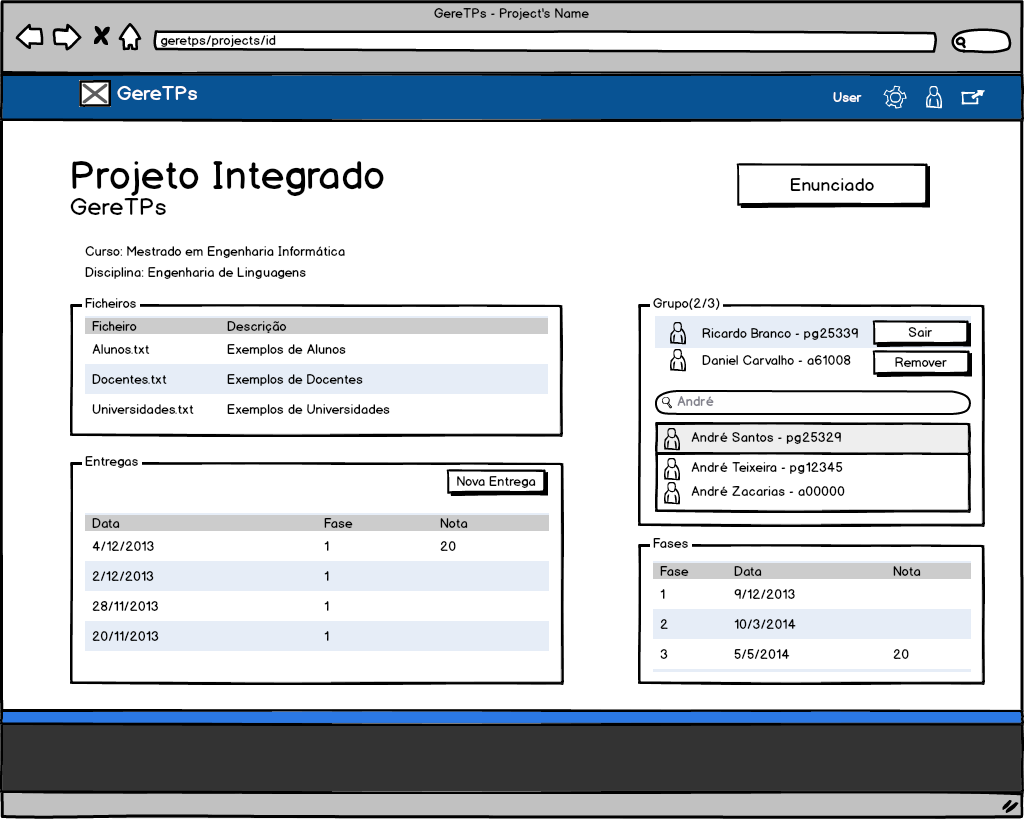
\includegraphics[width=1\textwidth]{images/prototipos/mockups/painelprojetoaluno.png}
         \caption{Painel de projeto de um aluno}
         \label{fig: painelprojetoaluno}
\end{figure}

Quando se visualiza um projeto, e de acordo com a Figura ~\ref{fig: projetoaluno}, pode-se aceder diretamente ao enunciado e relatório do projeto, ver e fazer \emph{Dowload} individual ou global(Ficheiro \emph{ZIP}) dos ficheiros submetidos, também é disponibilizado um resumo sob o trabalho feito, assim como a nota deste caso exista.Se for um docente responsável pela disciplina em que se enquadra o projeto a aceder à página, este pode fazer a avaliação do grupo, ou de cada membro individual e adicionar comentários sob a nota dada, tal como podemos ver na Figura ~\ref{fig: projetodocente}.\\

\begin{figure}[htbp]
        \centering
        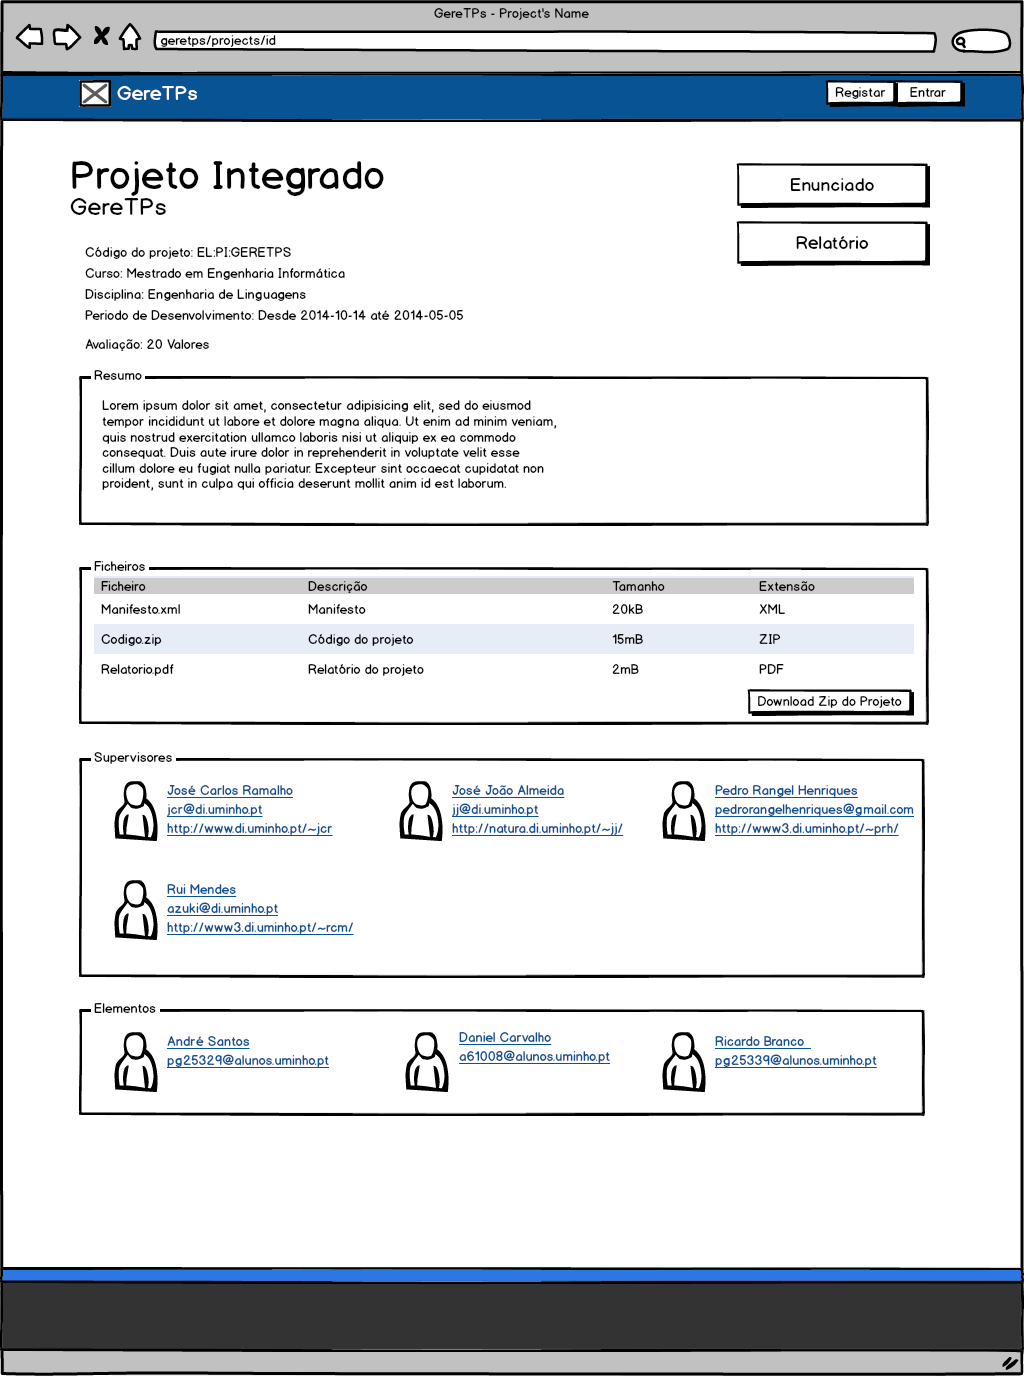
\includegraphics[width=1\textwidth]{images/prototipos/mockups/projetovisitante.png}
         \caption{Entrega vista por um visitante}
         \label{fig: projetoaluno}
\end{figure}

\begin{figure}[htbp]
        \centering
        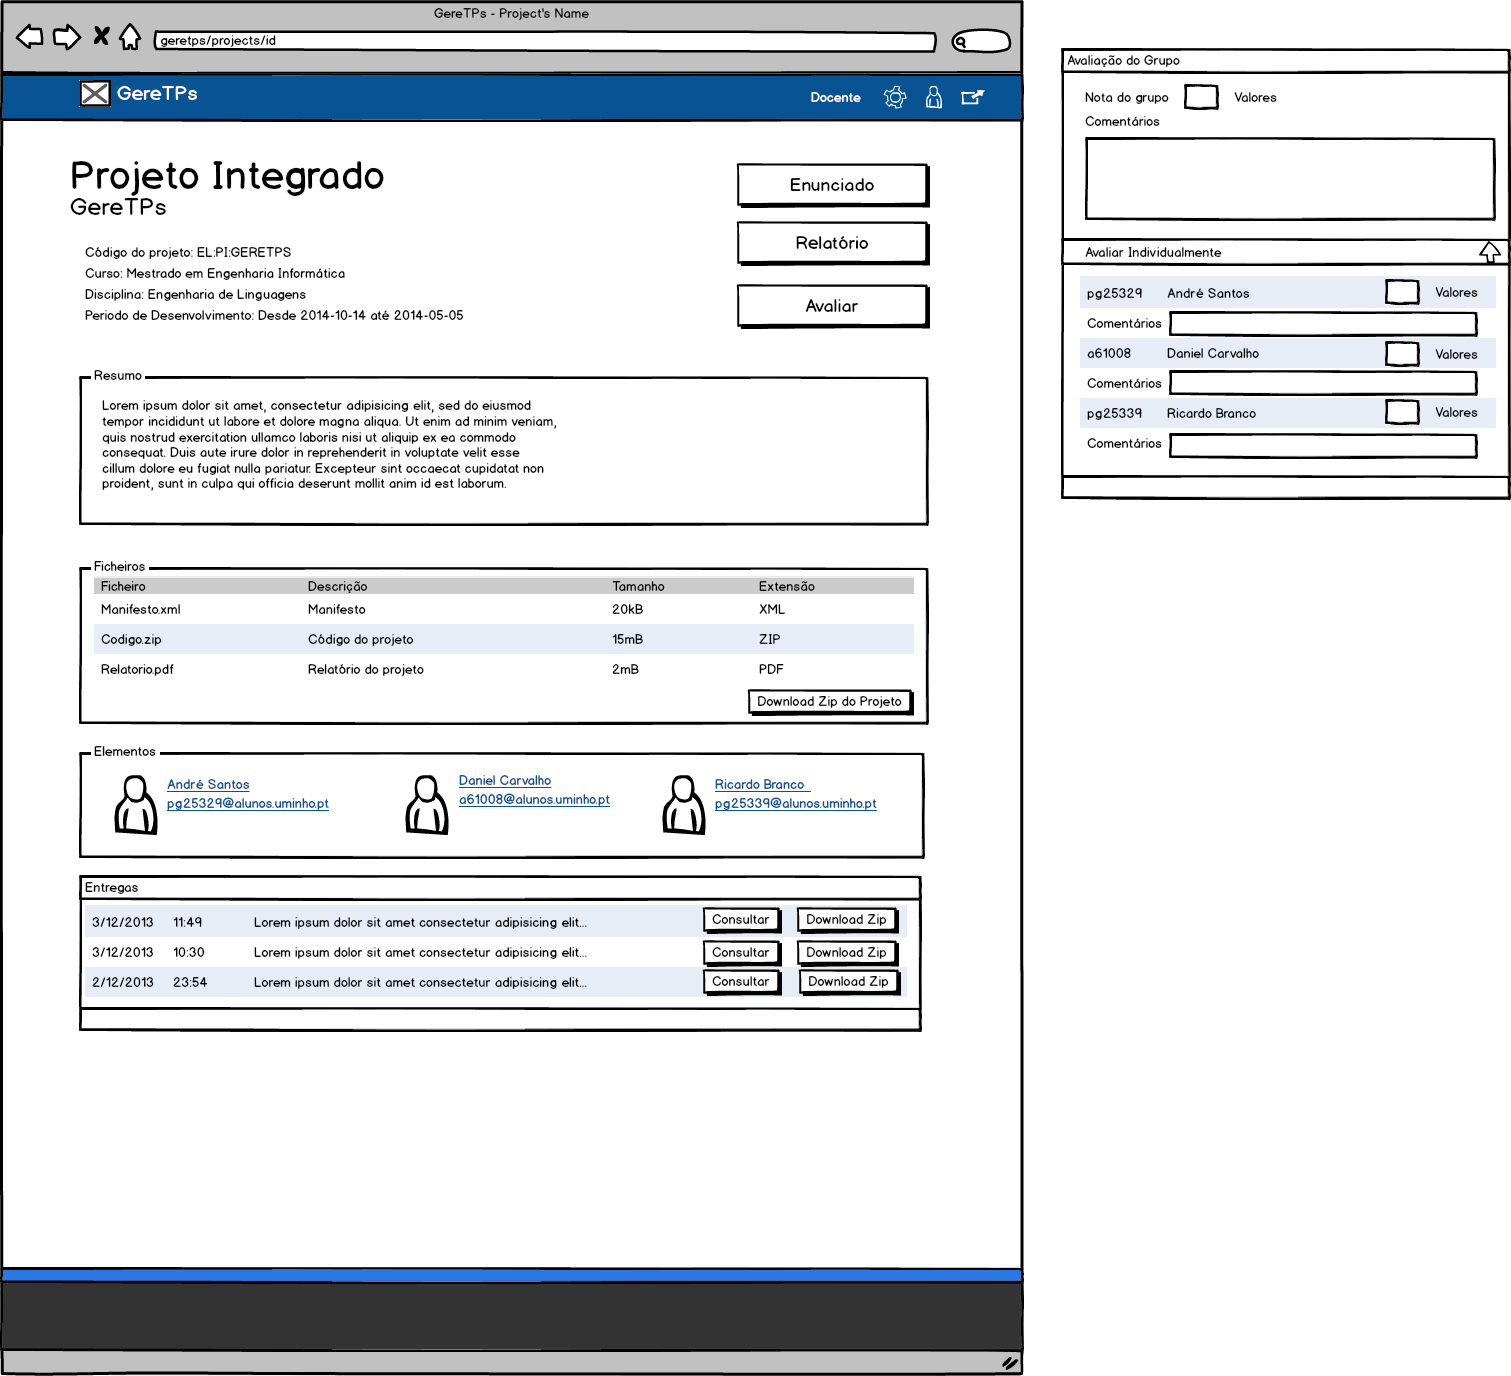
\includegraphics[width=1\textwidth]{images/prototipos/mockups/projetodocente.png}
         \caption{Entrega vista por um docente}
         \label{fig: projetodocente}
\end{figure}

\subsection{Protótipos fidedignos}
Para além dos primeiros protótipos, fizeram-se também protótipos fidedignos baseados nos anteriormente
citados de forma a aumentar o nível de detalhe, bem como aproximar a prototipagem o mais 
próximo possível do resultado final esperado. Assim sendo, segue-se na figura \ref{fig:prot_fid_home}
um exemplo da prototipagem fidedigna da página principal.
Com este tipo de protótipos espera-se aprimorar os detalhes, bem como os esquemas de cores,
arranjos gráficos, entre outros pormenores.
De notar que os protótipos fidedignos feitos neste projeto foram construídos diretamente a partir
da linguagem HTML.

\begin{figure}[H] 
  \centering
  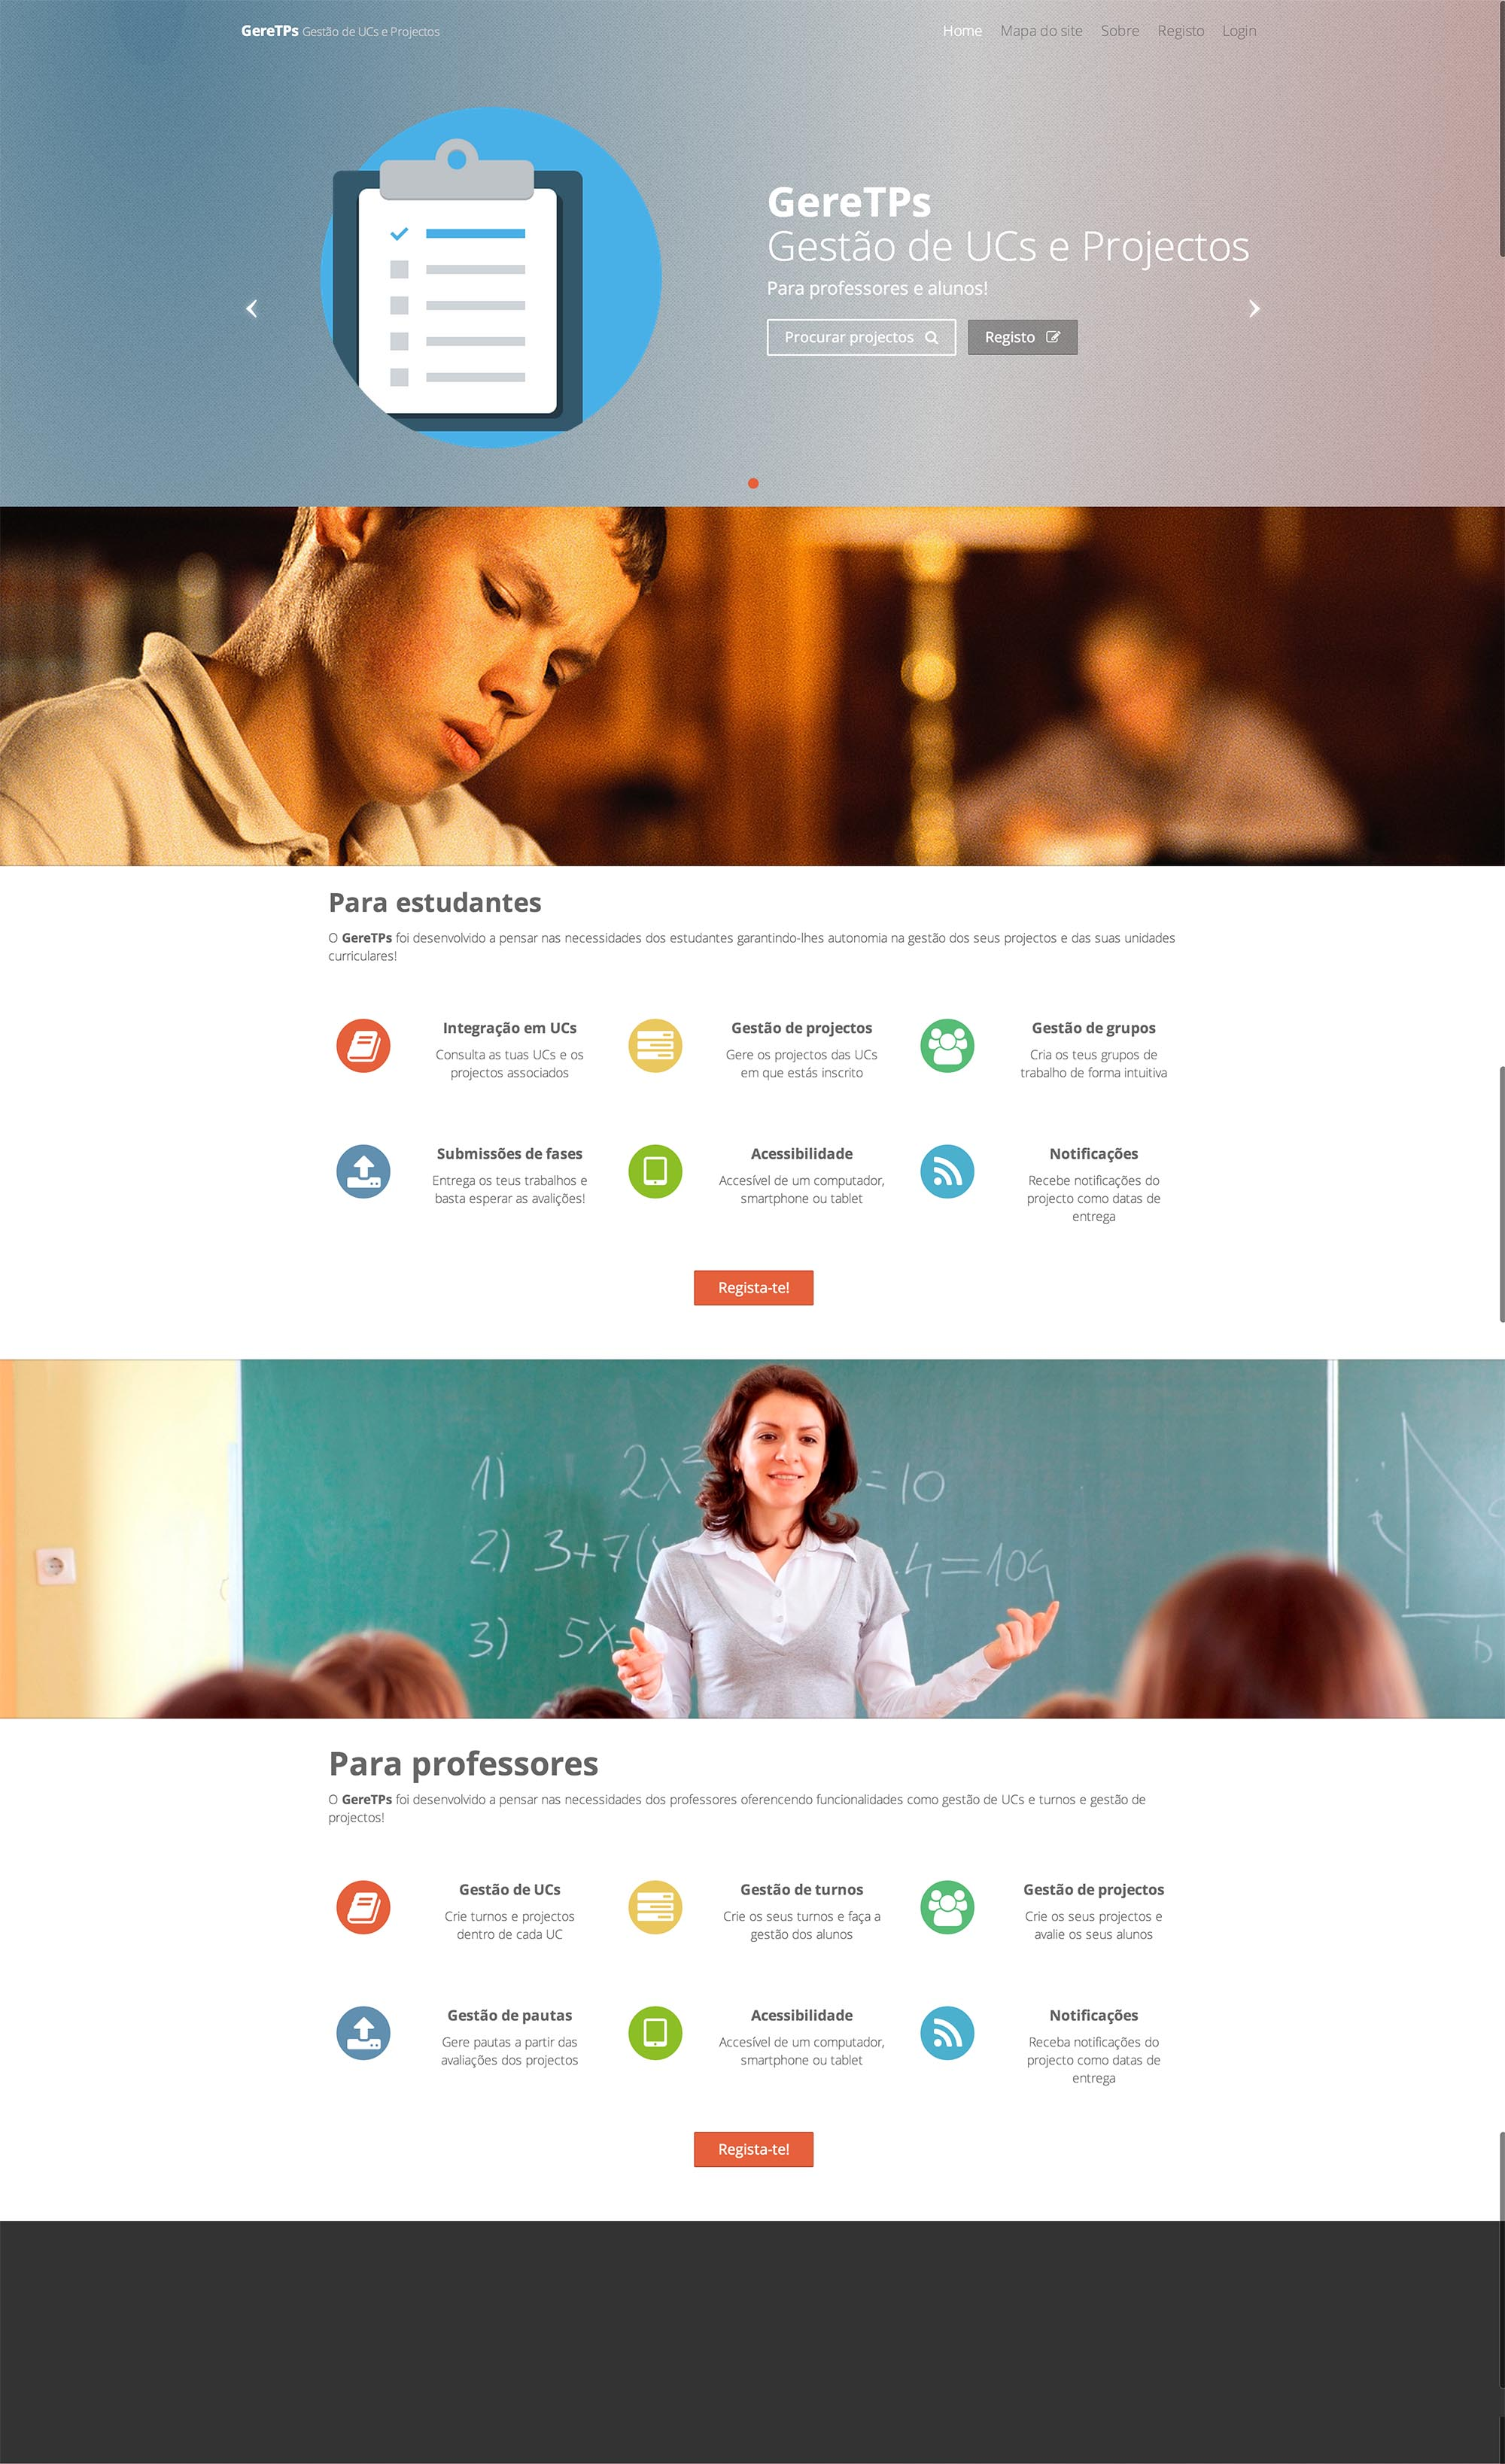
\includegraphics[width=0.8\textwidth,center]{images/prototipos/fidedigno_home.jpg}
  \caption{Protótipo fidedigno página inicial}
  \label{fig:prot_fid_home}
\end{figure}

\newpage


\section{Proposta tecnológica}

Para o desenvolvimento do nosso sistema, precisamos de combinar um vasto conjunto de tecnologias que permitam 
simplificar o desenvolvimento de todas as funcionalidades propostas.

De forma a organizar o fluxo de trabalho do grupo, utilizamos o \href{https://trello.com/}{\textbf{Trello}}, 
que é um sistema para gestão de tarefas que segue o método \textit{kanban}, muito usado no desenvolvimento com \textit{Scrum}. 

\begin{figure}[H] 
  \centering
  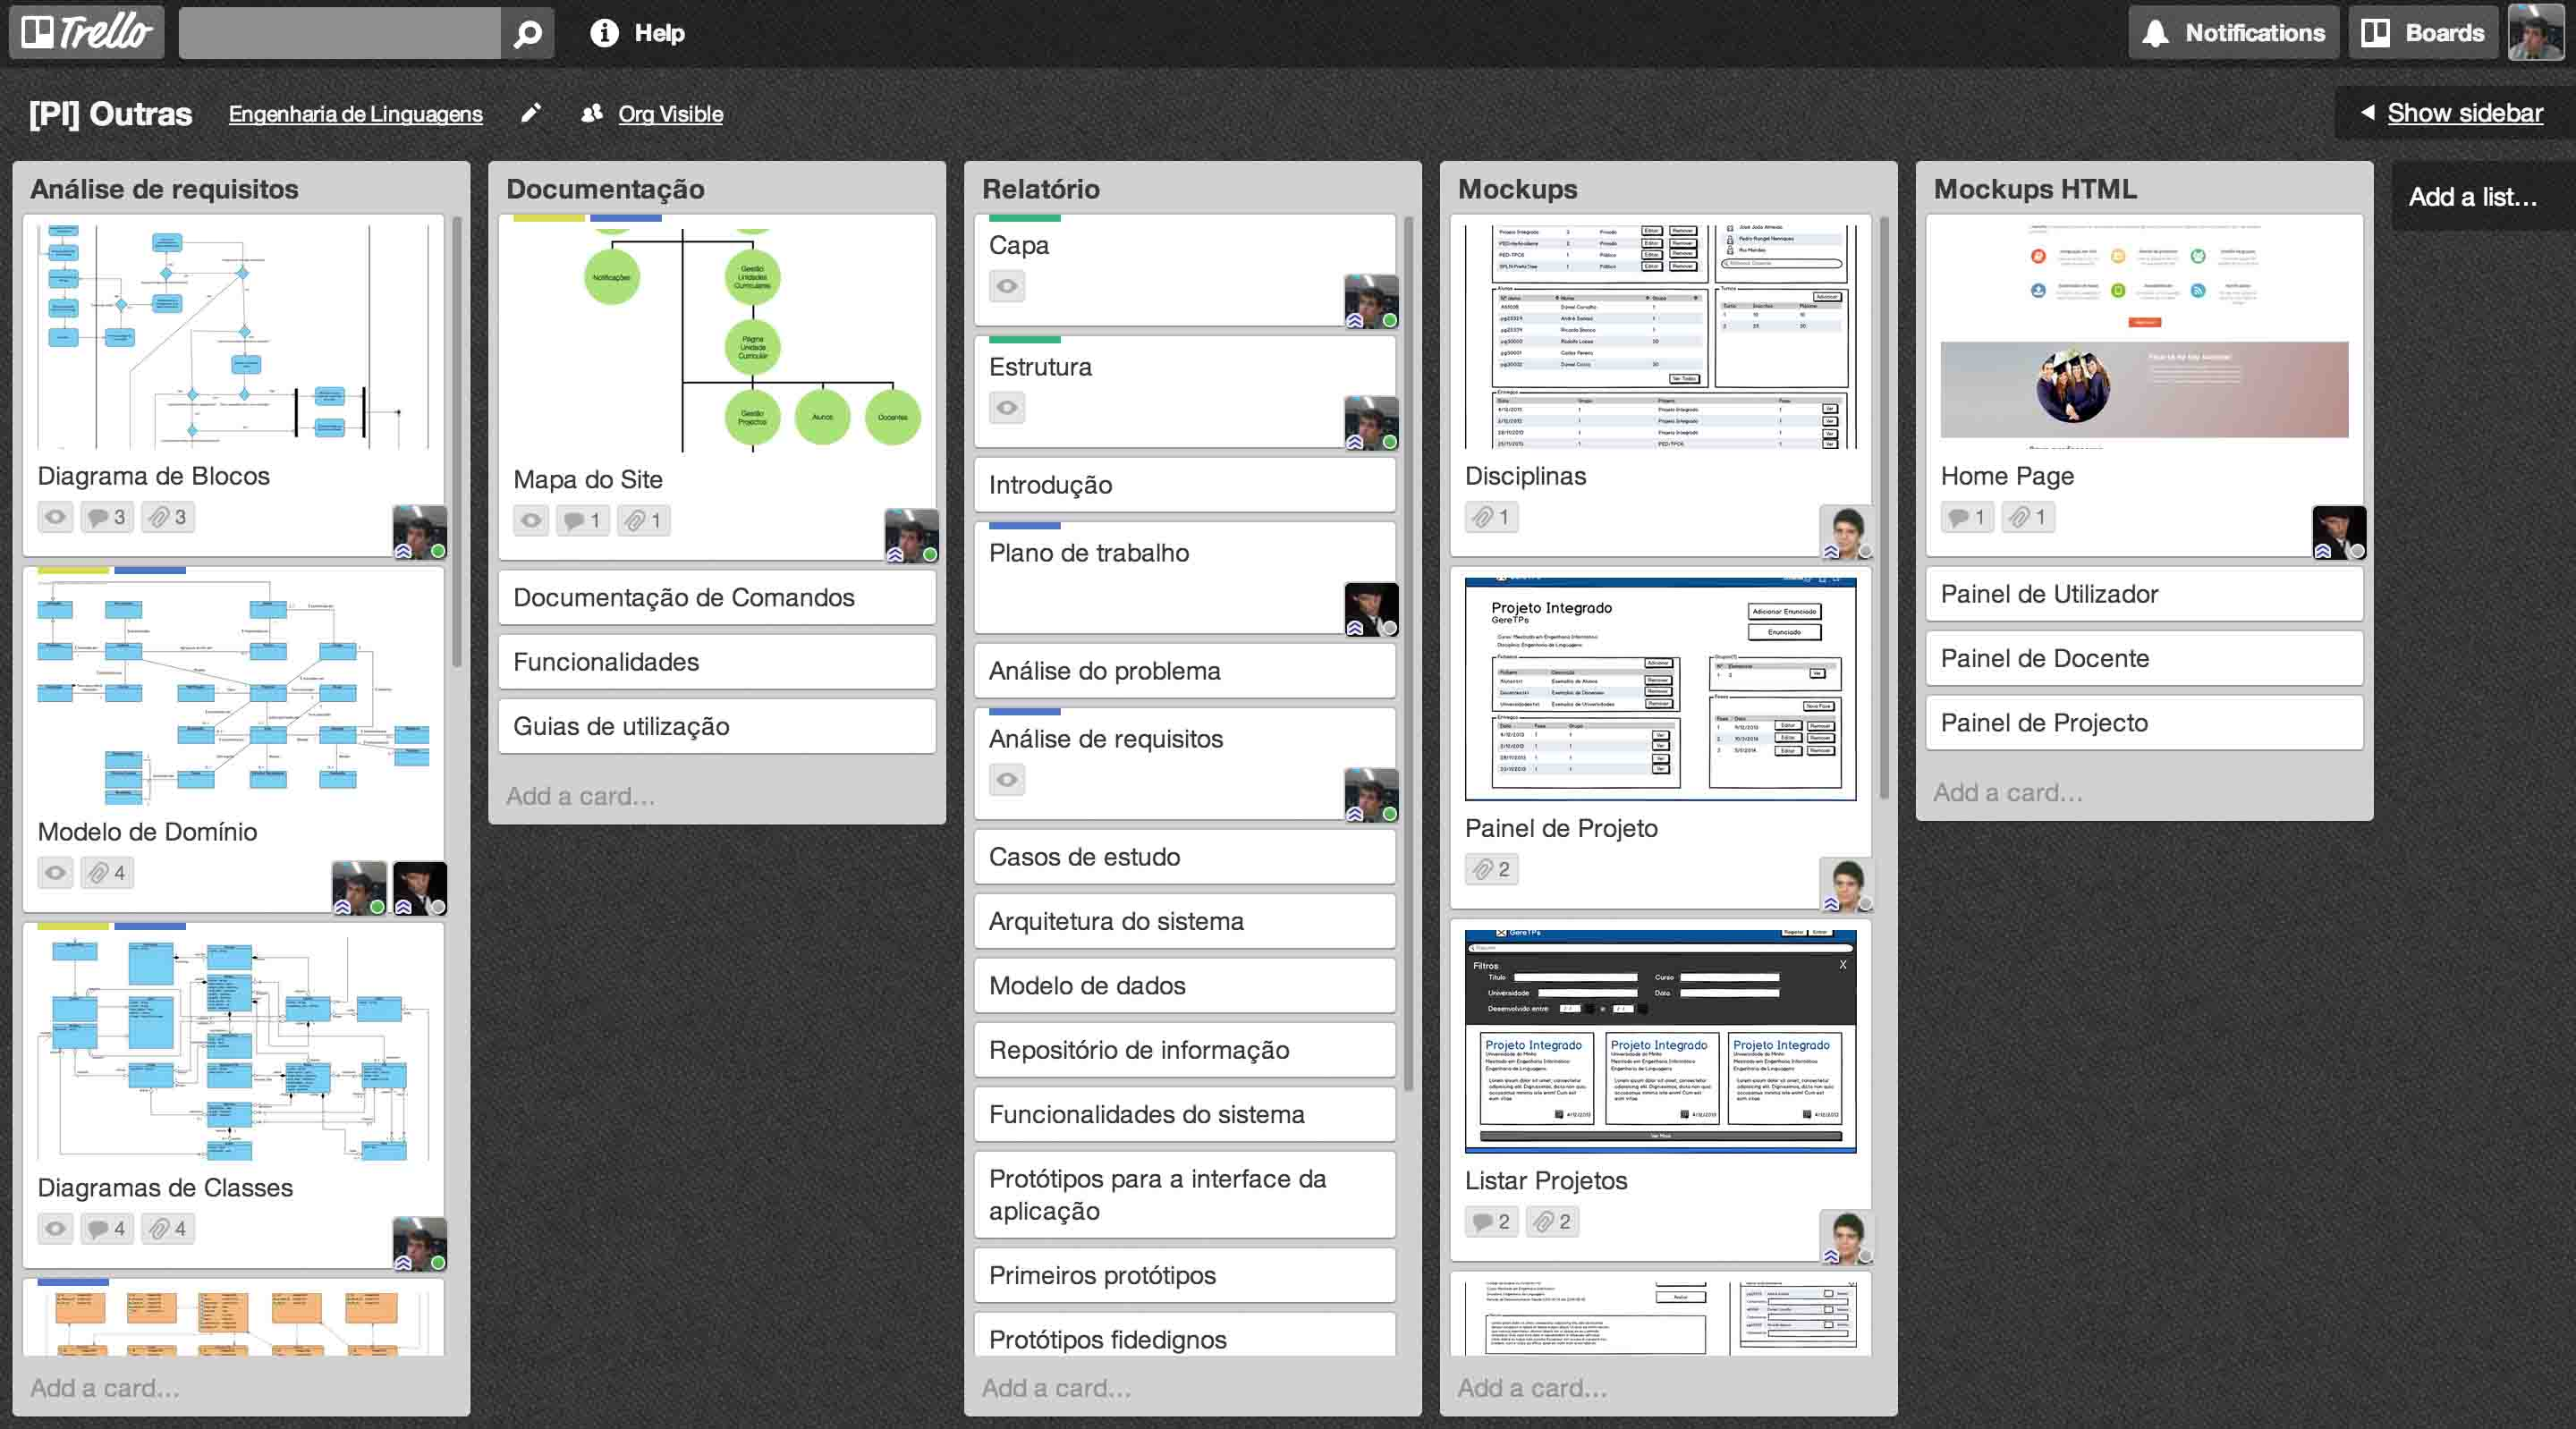
\includegraphics[width=1\textwidth]{images/tecnologias/trello}
  \caption{Trello}
  \label{fig:trello}
\end{figure}

Para o controlo de versões utilizaremos \textbf{Git}, que é um sistema de controlo de versões 
centralizado que apresenta as seguintes características:

\begin{itemize}
  \item Suporte consistente para desenvolvimentos não-lineares
  \item Desenvolvimento distribuído
  \item Compatibilidade com protocolos/sistemas existentes
  \item Manipulação eficiente de projetos extensos  
  \item Autenticação criptográfica do histórico 
  \item Modelo baseado em ferramentas 
  \item Estratégias de mescla (merge) conectáveis
  \item Empacotamento periódico explícito de objetos  
\end{itemize}

Para armazenar o código do nosso projeto vamos utilizar o \href{http://github.com}{\textbf{Github}}, 
que é um serviço de \textit{web hosting} o para projetos que usam o \textbf{Git} como sistema de controle de versões. 
Iremos utilizar um sistema de \textit{\textbf{Pull Requests}} e \textit{\textbf{Code Reviews}} 
para que assim todos os elementos possam ver e discutir o código produzido.

Procuraremos respeitar um dos fluxos de trabalho baseados em Git mais conhecidos, 
o \href{https://www.atlassian.com/git/workflows#!workflow-feature-branch}{\textbf{\textit{Feature Branch Workflow}}} 
que pode ser representado pela figura ~\ref{fig:git-workflow}.

\begin{figure}[H] 
  \centering
  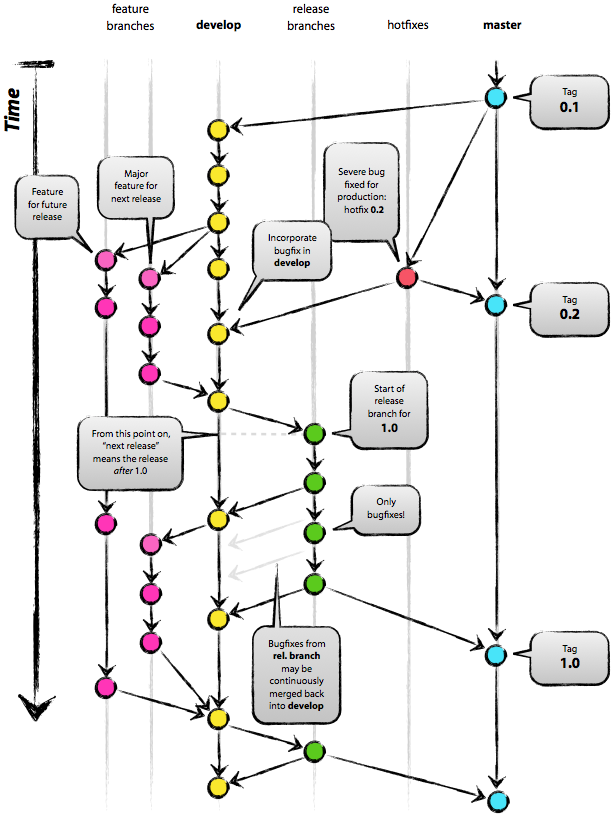
\includegraphics[width=0.5\textwidth]{images/tecnologias/git-workflow}
  \caption{Feature Branch Workflow}
  \label{fig:git-workflow}
\end{figure}

Rlativamente ao desenvolvimento, utilizaremos \href{http://rubyonrails.org/}{\textbf{Ruby on Rails}}, 
que é uma \textit{framework open-source} escrita em \textbf{Ruby}, otimizada para a produtividade sustentável. 
A \textit{framework} tem uma forte comunidade que defende conceitos como \textbf{DRY} \textit{(Don't Repeat Yourself)} 
e \textbf{\textit{Convention over configuration}}.

\textbf{Ruby on Rails} é uma \textit{meta-framework}, composta pelos seguintes \textbf{frameworks}:

\begin{description}[labelindent=1cm]
  \item[Active Record] Responsável pela interoperabilidade entre a aplicação e a base de dados, e pela abstração dos dados.
  \item[Action Pack] Compreende o \textbf{Action View} (gera o que o utilizador vê, como HTML, XML e JavaScript) 
  e o \textbf{Action Controller} (controle do fluxo de negócio).
  \item[Action Mailer] Responsável pelo serviço de entrega e receção de e-mails.
  \item[Active Support] Coleção de várias classes e bibliotecas, que foram considerados úteis para aplicações em Ruby on Rails.
\end{description}

Para além das \textit{frameworks} indicadas iremos recorrer a \textbf{Gems} para simplificar alguns processos, tais como:

\begin{description}[labelindent=1cm]
  \item[Devise] Autenticação de utilizadores.
  \item[Paperclip] Upload e validação de imagens e arquivos.
  \item[Capistrano] Automatização de processos de implantação \textit{(deployment)}.
  \item[Nokogiri] Parser de HTML e XML com XPath e seletores CSS.
  \item[XML-Simple] API simples para trabalhar com documentos XML.
\end{description} 

Pretendemos melhorar a nossa produtividade, e melhorar a legibilidade do código produzido utilizando os seguintes pré-processadores:

\begin{description}[labelindent=1cm]
  \item[\href{http://slim-lang.com/}{Slim}] para HTML.
  \item[\href{http://sass-lang.com/}{SASS}] para CSS.
  \item[\href{http://coffeescript.org/}{CoffeeScript}] para JavaScript.
\end{description} 

Utilizaremos também a \textit{framework} de \textit{front-end} \href{http://getbootstrap.com/}{\textbf{Twitter Bootstrap}} 
para ajudar a construirmos um serviço multi-plataforma e para reutilizarmos alguns componentes. 
E a biblioteca de Javascript \href{http://jquery.com/}{\textbf{JQuery}} para simplificar os \textit{scripts client side} que interagem com o HTML.\\

Para manipulação de documentos \textbf{XML}, utilizaremos as tecnologias lecionadas, tais como: \textbf{DTD}, \textbf{XSLT} e \textbf{XSD}.\\

Relativamente a tecnologias de Base de Dados, utilizaremos bases de dados SQL, mais especificamente \href{http://www.sqlite.org/}{\textbf{SQLite}} 
para ambientes de teste e desenvolvimento, e \href{http://www.postgresql.org/}{\textbf{PostgreSQL}} para ambientes de produção.




\section{Estado do desenvolvimento}
No sentido de colocar em prática todo o planeamento do desenvolvimento da 
aplicação seguiu-se de forma minimamente próxima o plano de trabalho já 
demonstrado na forma de diagramas de Gantt com pequenas alterações de prioridade 
no que diz respeito à implementação de algumas fases.
Nesse sentido após a construção da base da aplicação nas tecnologias que seriam 
usadas procedeu-se à prototipagem em HTML de algumas páginas. Neste momento 
é possível encontrar já em fase quase final a página principal da aplicação que sofreu 
algumas iterações até se aproximar do pretendido. Passado esta primeira fase de 
prototipagem começou-se por garantir a persistência de dados através da 
implementação do modelo de dados concebido durante a análise de requisitos bem 
como proceder à sua população com dados de teste.
No que diz respeito aos diferentes utilizadores das aplicação e à sua 
autenticação no sistema foram implementadas funcionalidades de registo e entrada 
no sistema de forma a garantir uma gestão fiel das funcionalidades que cada tipo 
de utilizador tem acesso, bem como garantir coerência de dados para cada 
utilizador individual. Após garantir a autenticação no sistema aos seus utilizadores,
 bem como o registo específico para cada um dos tipos de utilizadores (docentes e alunos), iniciou-se a
 implementação das funcionalidades básicas do sistema, nomeadamente o CRUD (create, read, update
 and delete) da aplicação, ou seja, a criação, leitura, actualização e remoção 
 de todas as entidades representadas no sistema (como por exemplo turnos, projectos, grupos, 
 avaliações, etc).
 Após uma implementação básica dessas funcionalidades decidimos iterar sobre as 
 funcionalidades ligadas ao tipo de utilizador aluno e refazê-las de raiz de forma a ir 
 de encontro ao que realmente são as funcionalidades que pretendemos 
 disponibilizar aos alunos da aplicação.
 Nesse sentido iniciou-se o desenvolvimento do painel do aluno que se torna o 
 centro de utilização da aplicação por parte deste tipo de utilizador. Aqui é 
 possível consultar os projetos em desenvolvimento por parte do utilizador, 
 assim como os projetos que se vão iniciar e os que já foram terminados. Também 
 é possível consultar as últimas notificações do sistema assim como se tornam 
 acessíveis todas as unidades curriculares em que cada aluno se encontra 
 inscrito. De seguida prosseguiu-se ao aprofundamento da implementação das funcionalidades sobre 
 projetos do lado do aluno, tendo sido desenvolvida uma página onde é possível 
 consultar as informações disponibilizadas para o projeto, bem como as fases, as 
 suas notificações, o grupo de trabalho e as últimas entregas. A partir daqui é 
 também possível consultar páginas de entregaa e fases de um projecto onde são 
 disponibilizadas informações como os ficheiros obrigatórios, a pauta de 
 avaliações, as entregas feitas e onde é possível efectuar novas entregas.
 Para além disso também se tornam acessíveis na página de um projecto páginas 
 que permitem a gestão de grupos e consulta de enunciados.
 Ainda do lado do aluno e no que diz respeito às unidades curriculares em que 
 estão inscritos é disponibilizada um página que permite a procura de unidades 
 curriculares e a sua inscrição mediante a aceitação por parte do docente do 
 respetivo pedido, bem como a funcionalidade de consulta das unidades 
 curriculares em que está inscrito e as que estão com a inscrição pendente, 
 assim com a opção para anular uma inscrição.
 Assim, é também tornada possível a consulta de todas as avaliações das 
 diferentes unidades curriculares em que um aluno se encontra inscrito.
 De referir que todas as funcionalidades que já foram implementadas já se 
 encontram numa fase de maturação considerável e que estão bastante próximas da sua 
 versão final apesar de estarem ainda sujeitas a pequenas alterações, tanto no sentido 
 do seu funcionamento como no sentido da própria interface, que por sua vez já se encontra preparada 
 para o acesso a partir de várioss tipos de dispositivos independentemente da resolução.
Em jeito de resumo já é possível fornecer aos alunos utilizadores do sistema uma 
aplicação que lhes permite gerir as suas unidades curriculares, ingressar em 
projectos, fazer entregas, consultar pautas e avalições, criar os seus grupos de trabalho, entre outras 
funcionalidades, garantido assim grande parte das funcionalidades planeadas para este tipo de 
utilizador. De seguida virar-se-ão as atenções para as funcionalidades no plano 
de utilização do sistema por parte dos docentes onde por agora se encontram 
implementadas funcionalidades básicas de CRUD.
\newpage

\section{Conclusão}
Chegando ao final da primeira fase deste projeto é possível destacar algumas conclusões e decisões
tomadas desde o início até ao ponto atual.

Relativamente ao levantamento de funcionalidades e análise de requisitos conseguiu-se retratar
corretamente o sistema em análise, cobrindo todo o espetro de funcionalidades necessárias para
o bom funcionamento da solução que se irá desenvolver para este problema de gestão de trabalhos 
práticos académicos em concreto.
Foram detetadas as principais necessidades dos diversos tipos de utilizadores 
para o qual este sistema é idealizado e também foi possível proceder a um 
planeamento bem definido no que diz respeito ao futuro do desenvolvimento deste 
projeto.

No que diz respeito às decisões tecnológicas foi decidido proceder à 
implementação da aplicação web usando a linguagem Ruby on Rails, não só pela 
experiência que os elementos do grupo já possuem com a respetiva 
\textit{framework}, mas também pelas suas características de prototipagem rápida 
e pelas filosofias de desenvolvimento que a regem.
Para além disso, a utilização desta framework irá ser bastante positiva no ponto 
em que se seguirá uma abordagem Agile no desenvolvimento de todo este sistema.

Por fim, a fase de desenvolvimento já foi iniciada e já foram criados vários prótotipos 
relativos às interfaces disponibilizadas para a interação entre os utilizadores 
e o sistema. Atualmente os resultados parecem ser positivos, pois a análise ao 
resultado destes protótipos relevam que estes se destacam pela simplicidade de 
intuitividade bastante elevada, o que é o objetivo idealizado para este 
sistema.

\newpage
\section{Anexos}
\begin{figure}[H] 
	\centering
	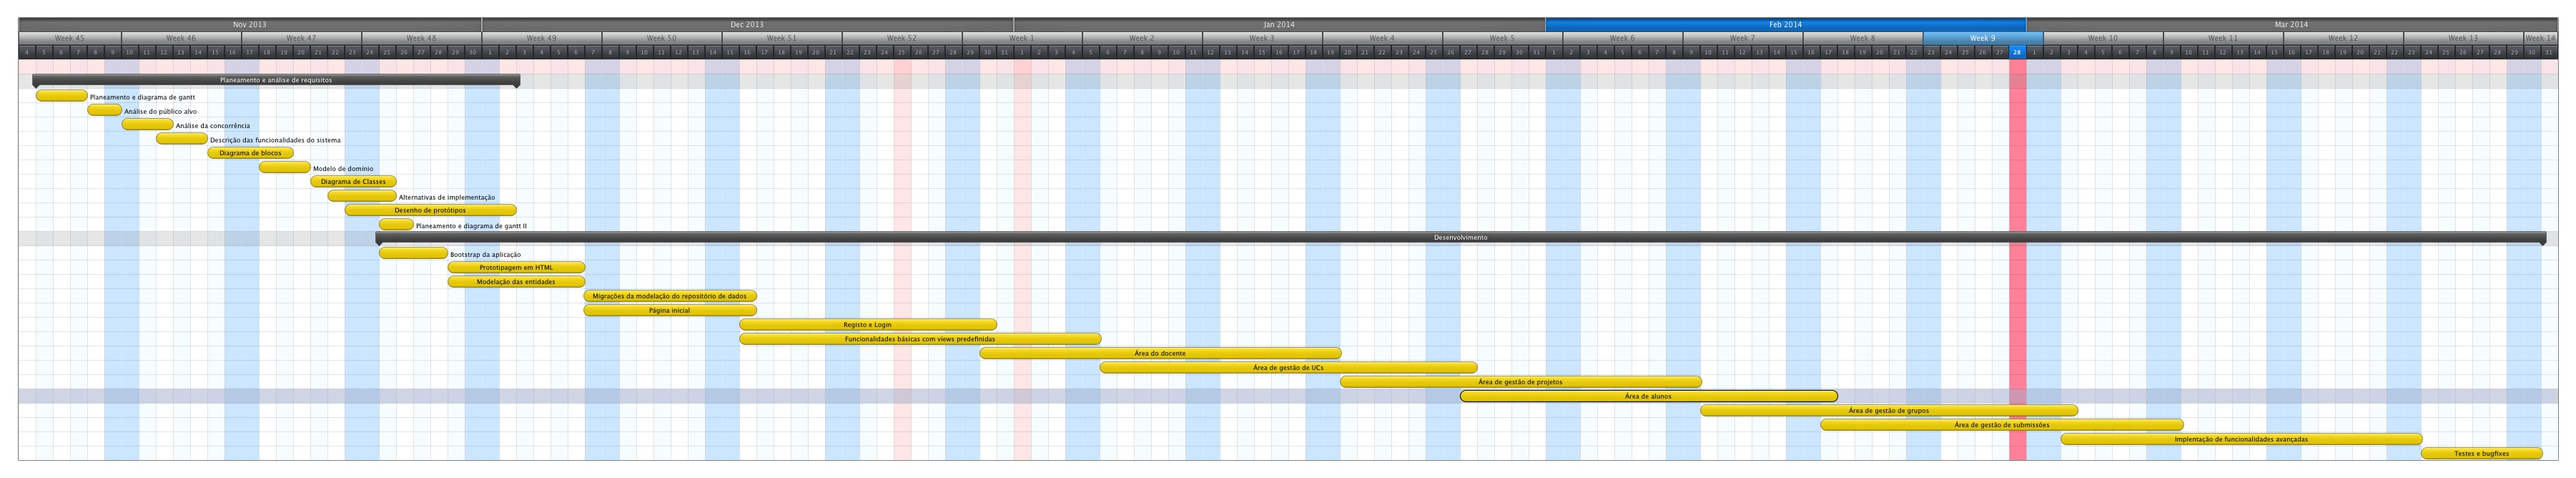
\includegraphics[width=0.3\textwidth]{images/plano_de_trabalho/gannt_0.png}
 	\caption{Diagrama de Gantt completo}
 	\label{fig: workplan0}
\end{figure}

\input{bibliografia}

\end{document}
